\documentclass[12pt,a4paper,oneside]{report}

% ============================================================
% Package configuration
% ============================================================

\usepackage[T1]{fontenc}
\usepackage[utf8]{inputenc}
\usepackage[english]{babel}
\usepackage{lmodern}

\usepackage{amsmath}
\usepackage{amssymb}
\usepackage{bm}
\usepackage{mathtools}

\usepackage[
  a4paper,
  top=2.5cm,
  bottom=2.5cm,
  left=2.5cm,
  right=2.5cm,
  headheight=26pt
]{geometry}

\usepackage{setspace}
\usepackage{booktabs}
\usepackage{array}
\usepackage{longtable}
\usepackage{graphicx}
\usepackage{caption}
\usepackage{float}
% Keeps a heading with the rows or lines that follow it.
\usepackage{needspace}
\usepackage{tikz}
\usetikzlibrary{arrows.meta, calc, positioning}

\usepackage{enumitem}
\usepackage{listings}
% Straight quotes in listings rather than the curly ones the text font gives.
\usepackage{upquote}
\usepackage{xcolor}
\usepackage{fancyhdr}
\usepackage{url}
\Urlmuskip=0mu plus 1mu
\urlstyle{same}
\usepackage[hidelinks]{hyperref}
\usepackage{cleveref}
\usepackage[numbers]{natbib}
\usepackage{siunitx}
\usepackage{amsthm}

% ============================================================
% Thesis settings
% ============================================================

\setstretch{1.5}
\setlength{\parindent}{0pt}
\setlength{\parskip}{0.35em}
\emergencystretch=2em

\setlist[itemize]{topsep=3pt, itemsep=2pt, parsep=0pt}
\setlist[enumerate]{topsep=3pt, itemsep=2pt, parsep=0pt}

\captionsetup{font=small, labelfont=bf, skip=6pt}
\graphicspath{{figures/}{figures/logos/}{plots/}}

\setlength{\headheight}{26pt}
\pagestyle{fancy}
\fancyhf{}
\fancyhead[L]{\small\nouppercase{\leftmark}}
\fancyfoot[C]{\thepage}
\renewcommand{\headrulewidth}{0.4pt}

\lstdefinestyle{cppstyle}{
  language=C++,
  basicstyle=\ttfamily\scriptsize\setstretch{0.9},
  keywordstyle=\color{blue!70!black}\bfseries,
  commentstyle=\color{gray!65}\itshape,
  stringstyle=\color{green!50!black},
  numbers=left,
  numberstyle=\tiny\color{gray!70},
  numbersep=5pt,
  frame=single,
  rulecolor=\color{gray!30},
  framerule=0.3pt,
  framesep=3pt,
  backgroundcolor=\color{gray!3},
  breaklines=true,
  breakatwhitespace=true,
  captionpos=t,
  columns=fullflexible,
  keepspaces=true,
  tabsize=2,
  showstringspaces=false,
  xleftmargin=1.2em,
  xrightmargin=0.2em,
  aboveskip=0.8em,
  belowskip=0.6em
}

\lstdefinestyle{pythonstyle}{
  language=Python,
  basicstyle=\ttfamily\scriptsize\setstretch{0.9},
  keywordstyle=\color{blue!70!black}\bfseries,
  commentstyle=\color{gray!65}\itshape,
  stringstyle=\color{green!50!black},
  numbers=left,
  numberstyle=\tiny\color{gray!70},
  numbersep=5pt,
  frame=single,
  rulecolor=\color{gray!30},
  framerule=0.3pt,
  framesep=3pt,
  backgroundcolor=\color{gray!3},
  breaklines=true,
  breakatwhitespace=true,
  captionpos=t,
  columns=fullflexible,
  keepspaces=true,
  tabsize=2,
  showstringspaces=false,
  xleftmargin=1.2em,
  xrightmargin=0.2em,
  aboveskip=0.8em,
  belowskip=0.6em
}

\newtheorem{remark}{Remark}[section]

% ============================================================
% Adaptive abbreviation handling
% ============================================================

\makeatletter

\newcommand{\DeclareThesisAcronym}[3]{%
  \expandafter\gdef\csname thesisacro@short@#1\endcsname{#2}%
  \expandafter\gdef\csname thesisacro@long@#1\endcsname{#3}%
}

\DeclareRobustCommand{\ThesisAcronymUsed}[1]{%
  \expandafter\gdef\csname thesisacro@used@#1\endcsname{}%
}

\DeclareRobustCommand{\UseThesisAcronym}[1]{%
  \if@filesw
    \begingroup
    \protected@write\@auxout{}{\string\ThesisAcronymUsed{#1}}%
    \endgroup
  \fi
}

\DeclareRobustCommand{\abbr}[1]{%
  \UseThesisAcronym{#1}%
  \@ifundefined{thesisacro@short@#1}{#1}{\csname thesisacro@short@#1\endcsname}%
}

\newcommand{\PrintThesisAcronym}[1]{%
  \@ifundefined{thesisacro@used@#1}{}{%
    \csname thesisacro@short@#1\endcsname
    & \csname thesisacro@long@#1\endcsname \\%
  }%
}

\DeclareThesisAcronym{DOF}{DOF}{Degree of Freedom}
\DeclareThesisAcronym{DH}{DH}{Denavit--Hartenberg}
\DeclareThesisAcronym{DLS}{DLS}{Damped Least Squares}
\DeclareThesisAcronym{ESTOP}{E-stop}{Emergency Stop}
\DeclareThesisAcronym{FCI}{FCI}{Franka Control Interface}
\DeclareThesisAcronym{FCU}{FCU}{Franka Control Unit}
\DeclareThesisAcronym{FK}{FK}{Forward Kinematics}
\DeclareThesisAcronym{FT}{F/T}{Force/Torque}
\DeclareThesisAcronym{HM}{HM}{Hochschule M\"unchen}
\DeclareThesisAcronym{IP}{IP}{Internet Protocol}
\DeclareThesisAcronym{MUAS}{MUAS}{Munich University of Applied Sciences}
\DeclareThesisAcronym{OS}{OS}{Operating System}
\DeclareThesisAcronym{PDF}{PDF}{Portable Document Format}
\DeclareThesisAcronym{PREEMPTRT}{PREEMPT\_RT}{Real-Time Preemption Patch}
\DeclareThesisAcronym{ROS}{ROS}{Robot Operating System}
\DeclareThesisAcronym{SE3}{SE(3)}{Special Euclidean Group in three dimensions}
\DeclareThesisAcronym{SO3}{SO(3)}{Special Orthogonal Group in three dimensions}
\DeclareThesisAcronym{SPD}{SPD}{Symmetric Positive Definite}
\DeclareThesisAcronym{SVD}{SVD}{Singular Value Decomposition}
\DeclareThesisAcronym{CSV}{CSV}{Comma-Separated Values}
\DeclareThesisAcronym{EE}{EE}{End-Effector}
\DeclareThesisAcronym{TCP}{TCP}{Tool Centre Point}
\DeclareThesisAcronym{TBM}{TBM}{Technische Berechnung und Simulation}

\makeatother

% ============================================================
% Commands and metadata
% ============================================================

\newcommand{\thesisTitleEnglish}{Design and Implementation of a Real-Time Impedance Controller for a 7-\abbr{DOF} Collaborative Robot}
\newcommand{\thesisTitleGerman}{Entwurf und Implementierung eines Echtzeit-Impedanzreglers f\"ur einen  7-achsigen kollaborativen Roboter}


\newcommand{\authorName}{Heykel Khadhraoui}
\newcommand{\matriculationNumber}{41192924}
\newcommand{\birthDatePlace}{[26.09.1995], [Tunis]}
\newcommand{\studyProgram}{Computational Engineering (M.Sc.)}
\newcommand{\studyGroup}{[Study group]}
\newcommand{\firstSupervisor}{Prof.\,Norbert Nitzsche}
\newcommand{\secondSupervisor}{Prof.\,Ruth Otto}
\newcommand{\issueDate}{1 May 2026}
\newcommand{\submissionDate}{1 November 2026}
\newcommand{\submissionPlace}{Munich}
\newcommand{\facultyEnglish}{Faculty of Mechanical, Automotive and Aeronautical Engineering}
%%\newcommand{\facultyGerman}{Fakult\"at f\"ur Maschinenbau, Fahrzeugtechnik, Luft- und Raumfahrttechnik}

\hypersetup{
  pdftitle={Design and Implementation of a Real-Time Impedance Controller for a 7-DOF Collaborative Robot},
  pdfauthor={\authorName},
  pdfsubject={Master's thesis in Computational Engineering}
}

\newcommand{\vx}{\mathbf{x}}
\newcommand{\vxd}{\dot{\mathbf{x}}}
\newcommand{\vxdd}{\ddot{\mathbf{x}}}
\newcommand{\vxDes}{\mathbf{x}_d}
\newcommand{\vxdDes}{\dot{\mathbf{x}}_d}
\newcommand{\vq}{\mathbf{q}}
\newcommand{\vqd}{\dot{\mathbf{q}}}
\newcommand{\vtau}{\bm{\tau}}
\newcommand{\vF}{\mathbf{F}}
\newcommand{\vp}{\mathbf{p}}
\newcommand{\vz}{\mathbf{z}}
\newcommand{\mJ}{\mathbf{J}}
\newcommand{\mR}{\mathbf{R}}
\newcommand{\mT}{\mathbf{T}}
\newcommand{\mK}{\mathbf{K}}
\newcommand{\mD}{\mathbf{D}}
\newcommand{\mM}{\mathbf{M}}
\newcommand{\mI}{\mathbf{I}}
\newcommand{\SO}{\UseThesisAcronym{SO3}\mathrm{SO}(3)}
\newcommand{\SE}{\UseThesisAcronym{SE3}\mathrm{SE}(3)}
\newcommand{\R}[1]{\mathbb{R}^{#1}}


% ============================================================
% Professor draft selection
% ============================================================
% Change only the true/false lines below.
% Example: use \ProfessorIncludeSystemSetuptrue to include Chapter 3,
% or \ProfessorIncludeSystemSetupfalse to exclude it.

\newif\ifProfessorIncludeTitlePage
\newif\ifProfessorIncludeDeclaration
\newif\ifProfessorIncludeAbstract
\newif\ifProfessorIncludeKurzfassung
\newif\ifProfessorIncludeTableOfContents
\newif\ifProfessorIncludeListOfFigures
\newif\ifProfessorIncludeListOfTables
\newif\ifProfessorIncludeAbbreviations
\newif\ifProfessorIncludeReferences

\ProfessorIncludeTitlePagetrue
\ProfessorIncludeDeclarationtrue
\ProfessorIncludeAbstracttrue
\ProfessorIncludeKurzfassungtrue
\ProfessorIncludeTableOfContentstrue
\ProfessorIncludeListOfFigurestrue
\ProfessorIncludeListOfTablestrue
\ProfessorIncludeAbbreviationstrue
\ProfessorIncludeReferencestrue

% Main thesis chapters
\newif\ifProfessorIncludeIntroduction
\newif\ifProfessorIncludeStateOfTheArt
\newif\ifProfessorIncludeSystemSetup
\newif\ifProfessorIncludeSoftwareImplementation
\newif\ifProfessorIncludeTheoreticalBackground
\newif\ifProfessorIncludeExperiments
\newif\ifProfessorIncludeConclusion

\ProfessorIncludeIntroductiontrue
\ProfessorIncludeStateOfTheArttrue
\ProfessorIncludeSystemSetupfalse
\ProfessorIncludeSoftwareImplementationfalse
\ProfessorIncludeTheoreticalBackgroundfalse
\ProfessorIncludeExperimentsfalse
\ProfessorIncludeConclusionfalse

% Appendices
\newif\ifProfessorIncludeAppendixA
\newif\ifProfessorIncludeAppendixB
\newif\ifProfessorIncludeAppendixC
\newif\ifProfessorIncludeAppendixD
\newif\ifProfessorIncludeAppendixE
\newif\ifProfessorIncludeAppendixF
\newif\ifProfessorIncludeAnyAppendix

\ProfessorIncludeAppendixAfalse
\ProfessorIncludeAppendixBfalse
\ProfessorIncludeAppendixCfalse
\ProfessorIncludeAppendixDfalse
\ProfessorIncludeAppendixEfalse
\ProfessorIncludeAppendixFfalse

\ifProfessorIncludeAppendixA\ProfessorIncludeAnyAppendixtrue\fi
\ifProfessorIncludeAppendixB\ProfessorIncludeAnyAppendixtrue\fi
\ifProfessorIncludeAppendixC\ProfessorIncludeAnyAppendixtrue\fi
\ifProfessorIncludeAppendixD\ProfessorIncludeAnyAppendixtrue\fi
\ifProfessorIncludeAppendixE\ProfessorIncludeAnyAppendixtrue\fi
\ifProfessorIncludeAppendixF\ProfessorIncludeAnyAppendixtrue\fi

\begin{document}

% These fallback labels keep chapter references readable when a related
% chapter is excluded from the professor draft.
\makeatletter
\newcommand{\ProfessorFallbackLabel}[3]{%
  \@ifundefined{r@#1}{\@namedef{r@#1}{{#2}{0}{#3}{}{}}}{}%
}
\ProfessorFallbackLabel{ch:intro}{1}{Introduction}
\ProfessorFallbackLabel{ch:literature}{2}{State of the Art}
\ProfessorFallbackLabel{ch:setup}{3}{System Setup}
\ProfessorFallbackLabel{ch:implementation}{4}{Software Implementation}
\ProfessorFallbackLabel{ch:theory}{5}{Theoretical Background}
\ProfessorFallbackLabel{ch:experiments}{6}{Experiments}
\ProfessorFallbackLabel{ch:conclusion}{7}{Conclusion}
\ProfessorFallbackLabel{sec:rt_kernel}{3.3}{Real-Time Ubuntu Kernel}
\ProfessorFallbackLabel{sec:exp_stability}{6.1}{Preliminary: Stability Analysis}
\ProfessorFallbackLabel{sec:future}{7.3}{Future Work}
\@ifundefined{r@sec:rt_kernel@cref}{%
  \@namedef{r@sec:rt_kernel@cref}{{[section][3][3]3.3}{[1][0][]0}{}{}{}}%
}{}%
\@ifundefined{r@sec:exp_stability@cref}{%
  \@namedef{r@sec:exp_stability@cref}{{[section][1][6]6.1}{[1][0][]0}{}{}{}}%
}{}%
\@ifundefined{r@sec:future@cref}{%
  \@namedef{r@sec:future@cref}{{[section][3][7]7.3}{[1][0][]0}{}{}{}}%
}{}%
\makeatother

\pagenumbering{Roman}

\ifProfessorIncludeTitlePage
  \hypersetup{pageanchor=false}
\begin{titlepage}
\pdfbookmark[0]{Title Page}{titlepage}
\thispagestyle{empty}

% Logo
\begin{flushleft}

\includegraphics[width=4.6cm]{figures/logos/hm-logo.png}
\end{flushleft}

\vspace{0.8cm}

\begin{center}

{\large\bfseries \thesisTitleEnglish \par}

\vspace{0.3cm}

{\large\itshape \thesisTitleGerman \par}

\vspace{1.1cm}

{\Large\bfseries Master Thesis}\\[0.35cm]
{\normalsize submitted for the degree of Master of Science (M.Sc.)}

\vspace{1.0cm}

{\normalsize submitted at}\\[0.15cm]
{\normalsize Hochschule M\"unchen}\\[0.15cm]
{\normalsize \facultyEnglish}

\vspace{1.0cm}

{\normalsize submitted by}\\[0.15cm]
{\large\bfseries \authorName}\\[0.15cm]
{\normalsize Study programme: \studyProgram}\\[0.15cm]
{\normalsize Matriculation number: \matriculationNumber}

\end{center}

\vfill

\noindent
\begin{tabular}{@{}p{4.2cm}p{10.2cm}@{}}
Main supervisor: & \firstSupervisor \\
Second supervisor: & \secondSupervisor \\
Issue date: & \issueDate \\
Submission date: & \submissionDate \\
\end{tabular}

\end{titlepage}

% Intentionally blank reverse of the title page.
\thispagestyle{empty}
\null
\clearpage
\hypersetup{pageanchor=true}

  \setcounter{page}{2}
\fi

\ifProfessorIncludeDeclaration
  \chapter*{Declaration of Authorship}
\addcontentsline{toc}{chapter}{Declaration of Authorship}

\noindent
I hereby declare that this master's thesis entitled

\begin{center}
\textit{``\thesisTitleEnglish''}
\end{center}

\noindent
was written independently and without assistance from third parties. All sources, references, software tools, and other resources used have been cited accordingly. This work has not previously been submitted as an examination requirement in this or any other form.

\vspace{1.2cm}

\noindent
{\large\bfseries Verfassererkl\"arung\par}

\vspace{0.5cm}

\noindent
Hiermit erkl\"are ich, dass ich die vorliegende Masterarbeit selbstst\"andig und ohne fremde Hilfe angefertigt habe. Alle verwendeten Quellen, Hilfsmittel, Softwarewerkzeuge und sonstigen Ressourcen wurden entsprechend angegeben. Die Arbeit wurde bisher keiner anderen Pr\"ufungsbeh\"orde in gleicher oder \"ahnlicher Form vorgelegt.

\vspace{3cm}

% The name and the signature share one right-aligned block, so the signature
% stays under the name whatever the name's width. The block is 5cm and the
% image 4cm, so an inset of 0.5cm would centre it; 0.9cm sits it 4mm to the
% right of centre. The \makebox fills the line so \centering cannot halve
% that inset.
\noindent
\submissionPlace, \declarationDate
\hfill
\begin{minipage}[t]{5cm}
  \centering
  \authorName\\[0.35cm]
  \makebox[\linewidth][l]{%
    \hspace*{0.9cm}
\includegraphics[width=4cm]{figures/signature.jpg}}
\end{minipage}\hspace{1cm}

% Intentionally blank reverse of the declaration page.
\clearpage
\thispagestyle{empty}
\null
\clearpage

  \clearpage
\fi

\ifProfessorIncludeAbstract
  \chapter*{Abstract}
\addcontentsline{toc}{chapter}{Abstract}

This thesis develops a real-time controller for a seven-degree-of-freedom
collaborative robot intended for surface grinding with a rectangular tool on a
planar surface. Cartesian impedance control is used to generate the required
pressing motion while allowing passive, contact-induced rotation of the tool
towards surface alignment. This behaviour is intended to reduce the effect of
angular mismatch at contact entry, which can otherwise produce edge-first
contact and increased contact loads.

Directional translational and rotational compliance was defined relative to the
surface. In addition, a virtual centre of compliance could be displaced from the
tool centre point to couple translational pressing with rotational motion and
thereby influence the preferred direction of alignment.

Surface-contact experiments investigated the angular-error component
about the first surface tangent relative to the calibrated surface.
Different stiffness and centre-of-compliance settings were compared.
Increasing rotational stiffness increased the angular error by about
\(276\,\%\), whereas the tested tangential translational stiffness variation
changed it by about \(4\,\%\) of the baseline error.
The effect of centre-of-compliance displacement depended on the entry
direction. The lowest measured mean error magnitudes were about
\(33\,\%\) and \(34\,\%\) below their respective tool-centre-point references,
at different tested positions.
The evaluated angular-error component could pass through zero.
Further contact-induced rotation could increase its final magnitude.

A separate pose-hold experiment evaluated the null-space controller. Projected
damping reduced cumulative joint motion by about \(25\,\%\), while
singular-value conditioning reduced the remaining net joint motion by
approximately \(99.8\,\%\) to \(99.9\,\%\).

\fi

\ifProfessorIncludeKurzfassung
  \chapter*{Kurzfassung}
\addcontentsline{toc}{chapter}{Kurzfassung}

\begin{otherlanguage}{ngerman}
% Keep the complete German summary on one page at the normal text size.
\setstretch{1.45}

Diese Arbeit entwickelt einen Echtzeitregler für einen siebenachsigen
kollaborativen Roboter zur Oberflächenbearbeitung mit einem rechteckigen
Werkzeug auf einer ebenen Fläche. Die kartesische Impedanzregelung erzeugt die
Anpressbewegung und ermöglicht eine passive,
kontaktinduzierte Drehung des Werkzeugs zur Ausrichtung an der Fläche. Dadurch
sollen die Auswirkungen einer Winkelfehlstellung bei Kontaktbeginn reduziert
werden, die andernfalls zu Kantenkontakt und erhöhten Kontaktlasten führen
kann.

Die translatorische und rotatorische Nachgiebigkeit wurde richtungsabhängig zur
Fläche definiert. Ein verschiebbares virtuelles Nachgiebigkeitszentrum koppelt
Anpressbewegung und Rotation. Seine Position relativ zum Werkzeugbezugspunkt
beeinflusst die bevorzugte Ausrichtungsrichtung.

In den Kontaktversuchen wurde die verbleibende Winkelfehlerkomponente um die
erste Flächentangente relativ zur kalibrierten Flächenreferenz untersucht.
Eine Erhöhung der Rotationssteifigkeit
vergrößerte den verbleibenden Fehler um etwa \(276\,\%\).
Die Variation der tangentialen Translationssteifigkeit veränderte ihn um etwa
\(4\,\%\) des Fehlers im Referenzfall.
Die Wirkung der Verschiebung hing von der Richtung des Fehlers bei
Kontaktbeginn ab.
Die kleinsten gemessenen mittleren Fehlerbeträge lagen bei unterschiedlichen
untersuchten Positionen etwa \(53\,\%\) und \(34\,\%\) unter den jeweiligen
Referenzwerten mit dem Nachgiebigkeitszentrum am Werkzeugbezugspunkt.
Die Winkelfehlerkomponente konnte ihr Vorzeichen wechseln. Weitere
kontaktinduzierte Drehung konnte ihren verbleibenden Betrag vergrößern.

In einem getrennten Posehalteversuch wurde die Nullraumregelung untersucht.
Die projizierte Dämpfung verringerte die kumulierte Gelenkbewegung gegenüber
der Einstellung ohne Nullraumdrehmoment um etwa \(25\,\%\).
Die Kombination aus Dämpfung und Singulärwertkonditionierung verringerte
die kumulierte Gelenkbewegung gegenüber der alleinigen Konditionierung
um etwa \(51\,\%\).

\end{otherlanguage}

\fi

\ifProfessorIncludeTableOfContents
  \tableofcontents
  \cleardoublepage
\fi

\ifProfessorIncludeListOfFigures
  \listoffigures
  \cleardoublepage
\fi

\ifProfessorIncludeListOfTables
  \listoftables
  \cleardoublepage
\fi

\ifProfessorIncludeAbbreviations
  \chapter*{List of Abbreviations}
\addcontentsline{toc}{chapter}{List of Abbreviations}
\markboth{List of Abbreviations}{List of Abbreviations}
\ReviewMark{green}{The abbreviations are separated from the symbol list and
their printed forms are controlled centrally.}

\renewcommand{\arraystretch}{1.2}

% All centrally declared abbreviations used by the thesis are printed.
% Keep this list alphabetical by short form.
\begin{longtable}{@{}ll@{}}
\PrintThesisAcronym{CSV}
\PrintThesisAcronym{DH}
\PrintThesisAcronym{DOF}
\PrintThesisAcronym{EE}
\PrintThesisAcronym{ESTOP}
\PrintThesisAcronym{FCI}
\PrintThesisAcronym{FCU}
\PrintThesisAcronym{FT}
\PrintThesisAcronym{IP}
\PrintThesisAcronym{LDLT}
\PrintThesisAcronym{OS}
\PrintThesisAcronym{PREEMPTRT}
\PrintThesisAcronym{ROS}
\PrintThesisAcronym{SE3}
\PrintThesisAcronym{SO3}
\PrintThesisAcronym{SVD}
\PrintThesisAcronym{TCP}
\end{longtable}

  \cleardoublepage
\fi

\pagenumbering{arabic}

\ifProfessorIncludeIntroduction
  \setcounter{chapter}{0}
  \chapter{Introduction}
\label{ch:intro}

Industrial manipulators are built to follow a commanded trajectory precisely,
and inside a structured cell that is sufficient. In surface-finishing
applications, however, the actual surface pose may differ from the programmed
pose because of placement tolerances: the surface is positioned by hand, the
tool is held in a gripper, and the residual angle between the two is not known
before contact. Under rigid position control, that initial angular deviation
cannot be absorbed by the motion and therefore generates high contact forces.

Collaborative robots make another option available, and they account for a
growing share of industrial deployments
\citep{IFR2023WorldRobotics,Villani2018HRC}. Joint torque sensing and a
torque-level command interface let the controller specify how the robot yields
under contact, not only where it goes. Three properties of the present
experimental arrangement shape what such a controller must achieve. The grinding
face is held in a gripper and is therefore not perfectly rigid with respect to
the end-effector. The surface plane is known only through a calibration that
carries its own uncertainty. The objective is consequently not force reduction
alone, but passive angular alignment of the tool during contact, measured
against a separately calibrated physical surface.

Impedance control specifies that yielding as a dynamic relation between motion
and interaction force \citep{Hogan1985}. Cartesian impedance control imposes
the relation at the end-effector, in task space, so compliance can be shaped
per direction rather than per joint. A contact task requires this compliance to
be direction dependent. A tool moved across a surface must hold its distance to
that surface, yet a small lateral misalignment should not build a large force.
Orientation behaves the same way: when a tilted tool edge meets the surface, the
contact wrench carries a moment as well as a force, and a stiffness matrix
chosen for the contact geometry admits a small rotation instead of resisting it.
The rotation that actually occurs during contact is the quantity this thesis
measures, which makes the stiffness and damping matrices a choice about contact
geometry and not only about free-space tracking.

That choice rests on three bodies of work. The first is Cartesian impedance
control itself. The controller rests on standard serial-manipulator kinematics
\citep{Siciliano2009,Craig2005,Murray1994}: homogeneous transformations for
pose, and the Jacobian for the velocity map. Khatib established the
operational-space formulation, in which a Cartesian wrench is mapped to joint
torques through \(J^\top\) \citep{Khatib1987}; that mapping is the one adopted
here. Hogan defined the impedance relation itself, between end-effector motion
and interaction force \citep{Hogan1985}. Ott et al.\ extended Cartesian
impedance control to flexible-joint robots, where joint elasticity limits the
stiffness the controller can actually realise \citep{Ott2008}, and
Albu-Sch\"affer et al.\ built the same law on joint-torque sensing
\citep{Albu2003}. The torque-sensing interface is the one this thesis uses; the
flexible-joint extension is not adopted, since joint elasticity is not modelled
here.

The second is the practice of running such a law in real time. Previous
Cartesian impedance implementations on the Franka Emika Panda discuss
requirements such as real-time model access, null-space control, signal
treatment, and command limiting \citep{Mayr2024CartesianImpedance}. The present
controller uses the libfranka model interface and includes a selectable
null-space torque. No separate application-level saturation of the Cartesian
wrench, joint torque, or torque rate was implemented, so the configured
robot-side collision monitoring remained the only independent mechanism for
terminating the motion when its thresholds were exceeded.

The third concerns where the compliance is centred. Fasse and Broenink
formulate spatial impedance about a selected point, so that translation and
rotation couple through its placement \citep{Fasse1997SpatialImpedance}. That
construction is the theoretical basis of the compliance-centre shift used here.
The same geometry appears mechanically in remote-centre-compliance devices for
assembly \citep{Nevins1989ComputerControlledAssembly,Watson1978RCC} and, more
recently, in flexure-based and variable-compliance-centre strategies for
peg-in-hole insertion, where the compliance is arranged so that contact forces
reduce rather than amplify misalignment
\citep{Wang2019VariableComplianceCenter,Hartisch2022FlexureRCC}. Those studies
mainly consider insertion, and they fix the compliance centre either through
mechanical design or through a strategy tuned for a hole. The effect of
independently varying the virtual compliance-centre position and the
axis-specific stiffness during planar tool alignment has received less
attention. This thesis investigates that effect using a software-defined
compliance centre on a torque-controlled robot, and measures what its placement
does to tool alignment against a surface.

The problem it addresses can be stated directly. The angular relation between
the tool and the surface plane is uncertain before contact, because both the
surface placement and the tool mounting carry tolerances, and under rigid
position control that residual angle produces an undesirable contact moment
rather than a corrective motion. A tool tilted with respect to the surface
cannot be brought flat by translational compliance alone: the wrench that closes
the gap must also carry a moment. Translational compliance therefore does not by
itself define the corrective rotation. Placing the centre of compliance away
from the TCP couples translation and rotation, so that pressing the tool into
the plane also rotates it toward the plane. The placement is a
task-to-impedance mapping, not a claim that the tool pivots about that point
physically, and the response it produces is therefore read from the motion
measured during contact.

The alignment response cannot be predicted from the gain values alone, because
it also depends on the contact geometry, the lever direction, the robot
configuration, and the compliance of the tool mounting. The experiments
therefore compare the effects of commanded tilt, directional stiffness, and
compliance-centre placement under otherwise matched conditions.
\Cref{ch:theory,ch:implementation} set out the frame conventions those
comparisons rely on.

\label{sec:objectives}
Within that scope, this work investigates how the commanded tilt, the rotational
and translational stiffness of each surface tangent, and the spatial position of
a virtual centre of compliance influence contact-induced alignment. The
controller is a phase-scheduled Cartesian impedance law, written in C++ with
libfranka and Eigen and running in the \(1\,\mathrm{kHz}\) torque loop of the
Franka Emika Panda. Torques are mapped with \(J^\top\), and Coriolis terms are
compensated from the model. Each phase carries its own Cartesian gains; damping
follows from a Cartesian-inertia estimate rather than being set by hand. A
surface frame carries the normal and the two tangents \(t_1\) and \(t_2\)
explicitly.

One run proceeds through fixed phases: the tool axis is aligned, the plane is
approached to a geometric clearance, the leading feature of the rectangular
tool face is selected, that feature is ramped into the surface, and tangential
grinding motion follows. During set-up, a compliance-centre \(6\times6\)
stiffness and damping matrix is shifted to the tool centre point (\abbr{TCP})
through an adjoint congruence. Its off-diagonal blocks are the
translation--rotation coupling this thesis measures.

The principal contributions are of two kinds. The following were implemented and
verified against the running controller:

\begin{itemize}
  \item A frame-consistent real-time Cartesian impedance controller for the
        7-\abbr{DOF} Panda.
  \item A spatial compliance-centre formulation within that controller, in which
        the \(6\times6\) stiffness and damping are shifted to the TCP.
  \item A calibrated contact methodology, in which the surface plane and the
        grinding-face axis are measured independently of each other.
\end{itemize}

The following were established experimentally:

\begin{itemize}
  \item Axis-specific measurement of the rotational and translational stiffness
        contributions to contact-induced alignment.
  \item Identification of the compliance-centre position as the parameter with
        the largest measured influence on alignment within the tested range,
        including the direction dependence of that influence: the lever
        direction that improves alignment is opposite for the two surface
        tangents.
\end{itemize}

One part of the implementation is deliberately excluded from both lists. The
projected joint damping and the two-point smallest-singular-value bias for the
redundant seventh joint complete the controller architecture, but no matched
comparison isolates their effect, so they are not claimed as experimentally
established. Full operational-space inverse dynamics, adaptive impedance,
online surface estimation, and claims concerning human safety are outside the
scope.

The remainder of the thesis follows the order of that investigation.
Chapter~\ref{ch:theory} sets out the impedance law, the frame conventions, and
the compliance-centre shift; Chapter~\ref{ch:implementation} gives their
real-time realisation on the Panda. Chapters~\ref{ch:methodology}
and~\ref{ch:results_discussion} describe the experimental methodology and
present the corresponding results. Chapter~\ref{ch:conclusion} states the
conclusions and the work that remains.

\fi

\ifProfessorIncludeStateOfTheArt
  \setcounter{chapter}{1}
  \chapter{State of the Art}
\label{ch:literature}

\section{Robot Kinematics and Dynamics}
\label{sec:lit_kinematics}

The kinematic and dynamic foundations of serial manipulators are treated
comprehensively in Siciliano et al.\ \cite{Siciliano2009}.
The book covers the Denavit--Hartenberg parameterisation, the geometric
and analytic Jacobian, operational-space dynamics, and redundancy
resolution, and is the standard graduate-level reference in the field.
Craig \cite{Craig2005} provides a complementary introduction that
emphasises homogeneous transformation matrices and forward kinematics;
its frame-convention notation is adopted throughout the present thesis.

Both references are textbooks.
Their treatment of impedance and force control is limited; for
contemporary results, primary literature must be consulted
\cite{Albu2003, Villani2016}.
A formal $SE(3)$ perspective on robot kinematics is given in
Murray et al.\ \cite{Murray1994}.

\section{Impedance Control: Origins and Development}
\label{sec:lit_impedance}

\subsection{Original Formulation}

Hogan \cite{Hogan1985} introduced the impedance control concept by
observing that a robot manipulator interacting with an environment is
best described not by prescribing a rigid trajectory but by specifying
a desired \emph{dynamic relationship} between force and motion.
He formulated this as a target impedance---a virtual mass-spring-damper
at the end-effector---and showed that it unifies position and force
control within a single framework.
This seminal contribution has been cited several thousand times and
remains the theoretical foundation of the present work.

\subsection{Operational-Space Formulation}

Khatib \cite{Khatib1987} developed the operational-space formulation,
in which the full robot dynamics are projected into Cartesian space.
He showed that Cartesian forces can be mapped to joint torques exactly
via the Jacobian transpose---the central equation $\bm{\tau}=\mathbf{J}^\top\mathbf{F}$
used in this thesis---and that the operational-space inertia matrix
can be used to decouple Cartesian axes dynamically.

\textbf{Critical assessment:} While Khatib's full dynamic formulation
yields theoretically superior decoupling, it requires accurate knowledge
of the robot's inertia matrix and introduces computational overhead.
In the present work the simplified quasi-static form is used
($\mathbf{M}=\mathbf{I}$), which is adequate at the low velocities
of the virtual wall task and avoids the sensitivity to model errors
inherent in the dynamic inversion.

\subsection{Admittance Control: An Alternative Approach}

A closely related alternative is \textbf{admittance control}, in which
an outer position/velocity loop receives a force measurement and
generates a modified position reference for an inner position
controller.
Unlike impedance control, admittance control can be layered on top of
any existing position-controlled robot and does not require torque
control capability.
However, it introduces an additional control loop with its own bandwidth
limitation and typically requires an external force/torque sensor.

The Panda's integrated joint torque sensing and FCI torque-control mode
make direct impedance control---as implemented in this thesis---the
more natural and lower-latency choice for this platform.

\subsection{Variable-Impedance and Adaptive Approaches}

Recent research has explored impedance controllers with
\emph{variable} stiffness and damping, adjusted online based on
task requirements or estimated interaction forces.
These approaches improve performance across a wider range of tasks
but introduce stability risks if the parameter update law is not
carefully designed.
The present thesis uses fixed impedance parameters, which guarantees
stability via the Lyapunov argument of \cref{sec:exp_stability} and
is sufficient for the virtual wall task.
Variable-impedance extension is identified as future work in
\cref{sec:future}.

\section{Franka Emika Platform and libfranka}
\label{sec:lit_franka}

The Franka Control Interface \cite{FCI2023} exposes a deterministic
1\,kHz torque-control loop via the open-source \texttt{libfranka}
C++ library.
Unlike ROS-based frameworks, libfranka provides direct access to
joint states, the geometric Jacobian, and model quantities (gravity,
Coriolis, mass matrix) without any middleware overhead.

\textbf{Critical assessment:} The libfranka model is computed from
nominal robot parameters identified by the manufacturer.
For the impedance tasks considered in this thesis (low velocity,
no payload), the model accuracy is sufficient.
Payloads or high-speed motions would require re-identification of
the dynamic parameters.

The FCI imposes a strict 1\,ms callback deadline; violation triggers
an immediate safety halt.
This makes real-time Linux a prerequisite, as documented in
\cref{sec:rt_kernel}.

\section{Summary and Positioning of This Work}
\label{sec:lit_summary}

\cref{tab:lit_comparison} summarises the approaches reviewed above and
positions the present thesis within this landscape.

\begin{table}[htb]
\centering
\caption{Comparison of Cartesian compliance approaches.}
\label{tab:lit_comparison}
\renewcommand{\arraystretch}{1.4}
\begin{tabular}{@{}p{3.2cm}p{2.8cm}p{2.8cm}p{3.5cm}@{}}
\toprule
Approach & Force sensor needed & Requires torque control & Used in this thesis \\
\midrule
Admittance control & Yes & No & No \\
Impedance control (dynamic) & No & Yes & Partial ($\mathbf{M}=\mathbf{I}$) \\
Impedance control (quasi-static) & No & Yes & \textbf{Yes} \\
Variable impedance & Optional & Yes & No (future work) \\
\bottomrule
\end{tabular}
\end{table}

The quasi-static Cartesian impedance controller implemented in this
thesis represents the best trade-off between implementation complexity,
stability guarantees, and suitability for the Panda platform.
The closest related experimental work is Albu-Sch\"affer and Hirzinger
\cite{Albu2003}, who implemented Cartesian impedance control on the
DLR light-weight robot with a similar Jacobian-transpose approach;
their stability analysis corroborates the Lyapunov argument of
\cref{sec:exp_stability}.
A unified treatment of impedance and admittance control is given by
Ott et al.\ \cite{Ott2008}.

%% =============================================================
%%  CHAPTER 3: SYSTEM SETUP AND COMMISSIONING
%% =============================================================

\fi

\ifProfessorIncludeSystemSetup
  \setcounter{chapter}{2}
  \chapter{System Setup and Commissioning}
\label{ch:setup}

Before the impedance controller can be executed on the Franka Emika Panda,
the complete hardware and software environment must be correctly configured.
This chapter covers the setup of the workstation, network connection,
Franka Desk and FCI access, real-time Ubuntu kernel, libfranka installation,
and C++ build environment, as specified in Objective~2 of the thesis
registration.

\section{Hardware Architecture and Network Connection}
\label{sec:hw_network}

The experimental platform consists of the Panda arm, its Franka Control
Unit (FCU), a workstation PC, and an emergency stop device.
The workstation is connected \textbf{directly} to the FCI Ethernet port
of the FCU with a Cat\,6a cable---no intermediate switch is permitted,
as any additional hop introduces latency sufficient to trigger an FCI
communication timeout.

Static IP addresses are assigned:

\begin{center}
\begin{tabular}{@{}lll@{}}
\toprule
Device & Interface & Address \\
\midrule
FCU (FCI port) & \texttt{eth0} & \texttt{172.16.0.2} \\
Workstation    & \texttt{eth1} & \texttt{172.16.0.1/24} \\
\bottomrule
\end{tabular}
\end{center}

Connectivity is verified with \texttt{ping 172.16.0.2}; the round-trip
time must be consistently below $1\,\mathrm{ms}$.

\section{Franka Desk and FCI Access}
\label{sec:franka_desk}

Franka Desk is the web-based configuration interface, accessible
at \url{https://172.16.0.2} from any browser on the workstation.
Before real-time torque commands can be sent, the following steps are
required:

\begin{enumerate}
  \item Unlock the robot joints via the Franka Desk \textit{Joints} page.
  \item Activate FCI mode in \textit{Settings} $\to$ \textit{Network}.
  \item Confirm that no error is shown on the status indicator.
  \item Place the emergency stop within reach of the operator.
\end{enumerate}

All experiments are conducted with FCI active and the emergency stop
accessible at all times.

\section{Real-Time Ubuntu Kernel}
\label{sec:rt_kernel}

The FCI requires that the control callback completes within 1\,ms.
A standard Linux kernel cannot guarantee this because high-priority threads
can be preempted by interrupt handlers.
The PREEMPT\_RT patch makes all kernel threads and interrupt handlers fully
preemptible, reducing worst-case scheduling latency to below $50\,\mu s$.

Installation steps:

\begin{enumerate}
  \item Install Ubuntu 22.04 LTS on the workstation.
  \item Download and apply the PREEMPT\_RT patch for the corresponding
        kernel version.
  \item Compile and install the patched kernel:
        \texttt{make -j\$(nproc) deb-pkg}.
  \item Grant real-time scheduling priority to the control user:
        add \texttt{@realtime soft rtprio 99} to
        \texttt{/etc/security/limits.conf}.
  \item Set CPU governor to performance:
        \texttt{cpufreq-set -g performance}.
\end{enumerate}

The maximum latency of the patched system is verified with
\texttt{cyclictest}, which must show a worst-case latency below
$200\,\mu s$ under load before any FCI experiments are conducted.

\section{libfranka Installation}
\label{sec:libfranka}

\texttt{libfranka} is built from source to match the firmware version of
the robot controller:

\begin{lstlisting}[style=cppstyle, language=bash,
  caption={Build and install libfranka from source},
  label={lst:libfranka}]
sudo apt install build-essential cmake git libpoco-dev libeigen3-dev
git clone --recursive https://github.com/frankaemika/libfranka
cd libfranka && git checkout 0.9.2
mkdir build && cd build
cmake -DCMAKE_BUILD_TYPE=Release -DBUILD_TESTS=OFF ..
cmake --build . -j$(nproc)
sudo make install
\end{lstlisting}

The installation is verified by running the
\texttt{communication\_test} example program provided with libfranka,
which must report zero packet losses over a 60-second run.

\section{C++ Build Environment}
\label{sec:cpp_env}

All controller code is built with CMake in Release mode (\texttt{-O3}),
which provides approximately three times faster matrix operations compared
to Debug mode.
The following libraries are required:

\begin{itemize}
  \item \textbf{Eigen\,3}: header-only linear algebra library for all
        matrix and vector operations.
  \item \textbf{libfranka}: robot communication and model interface.
  \item \textbf{Poco}: network and threading utilities (dependency of
        libfranka).
\end{itemize}

A minimal \texttt{CMakeLists.txt}:

\begin{lstlisting}[style=cppstyle, language=bash,
  caption={Minimal CMakeLists.txt for a libfranka controller},
  label={lst:cmake}]
cmake_minimum_required(VERSION 3.10)
project(impedance_controller)
set(CMAKE_CXX_STANDARD 14)
set(CMAKE_BUILD_TYPE Release)
find_package(Franka REQUIRED)
find_package(Eigen3 REQUIRED)
add_executable(impedance_ctrl src/impedance_controller.cpp)
target_link_libraries(impedance_ctrl Franka::Franka Eigen3::Eigen)
\end{lstlisting}

%% =============================================================
%%  CHAPTER 4: SOFTWARE IMPLEMENTATION
%% =============================================================

\fi

\ifProfessorIncludeSoftwareImplementation
  \setcounter{chapter}{3}
  \chapter{Software Implementation}
\label{ch:implementation}

This chapter describes the modular C++ software structure developed for
reading robot states, accessing model information, and executing the
impedance controller in a reproducible manner, addressing Objective~3
of the thesis registration.

\section{Software Architecture}
\label{sec:sw_arch}

The software is structured in three layers, illustrated in
\cref{fig:sw_arch}:

\begin{enumerate}
  \item \textbf{Communication layer}: establishes and maintains the
        1\,kHz \abbr{FCI} connection via \texttt{libfranka}.
  \item \textbf{State and model layer}: reads joint positions, velocities,
        and the Jacobian; retrieves gravity and Coriolis vectors from the
        robot model.
  \item \textbf{Control layer}: evaluates the impedance law and returns
        joint torques within the 1\,ms deadline.
\end{enumerate}

\begin{figure}[htb]
\centering
\begin{tikzpicture}[
  box/.style={draw, rounded corners=3pt, minimum width=4.2cm,
               minimum height=0.9cm, align=center, font=\small},
  arr/.style={-{Latex}, thick}
]
  \node[box, fill=blue!10]  (hw)    at (0, 0.0) {Franka Panda\\(Hardware)};
  \node[box, fill=orange!15](fci)   at (0,-1.8) {\abbr{FCI} / \texttt{libfranka}};
  \node[box, fill=green!10] (state) at (0,-3.6) {State \& Model Layer\\($\mathbf{T}_e$, $\mathbf{J}$, $\bm{\tau}_g$)};
  \node[box, fill=red!10]   (ctrl)  at (0,-5.4) {Control Layer\\$\bm{\tau}=\mathbf{J}^\top\mathbf{F}$};
  \draw[arr] (hw)    -- (fci)   node[midway,right,font=\tiny]{1\,kHz};
  \draw[arr] (fci)   -- (state) node[midway,right,font=\tiny]{robot state};
  \draw[arr] (state) -- (ctrl)  node[midway,right,font=\tiny]{$\vq,\mathbf{T}_e,\mathbf{J}$};
  \draw[arr] (ctrl.east) -- ++(1.5,0) |- (fci.east)
    node[pos=0.25,right,font=\tiny]{$\bm{\tau}_{\mathrm{cmd}}$};
\end{tikzpicture}
\caption{Three-layer software architecture. The control layer evaluates
         the impedance law and returns joint torques to the FCI
         within the 1\,ms deadline.}
\label{fig:sw_arch}
\end{figure}

\section{State Acquisition and Model Access}
\label{sec:state_model}

Each 1\,ms control cycle extracts the following from
\texttt{franka::RobotState}:

\begin{itemize}
  \item \texttt{state.q}/\texttt{state.dq}: $\vq$ and $\vqd$.
  \item \texttt{state.O\_T\_EE}: $\mathbf{T}_e\in \SE$
        as a $4\times4$ column-major array of 16 doubles.
  \item \texttt{model.zeroJacobian(...)}: the $6\times7$ geometric
        Jacobian $\mathbf{J}(\vq)$ in the base frame.
  \item \texttt{state.gravity}: the $7\times1$ gravity vector
        $\bm{\tau}_g(\vq)$.
  \item \texttt{state.coriolis}: the $7\times1$ Coriolis vector
        $\bm{\tau}_c(\vq,\vqd)$.
\end{itemize}

\section{Control Loop Implementation}
\label{sec:control_impl}

The complete impedance control loop is implemented as a \texttt{libfranka}
torque callback.
The callback receives the current robot state and must return a
\texttt{franka::Torques} object within 1\,ms.
The following listing shows the full implementation as deployed in the
experiments:

\begin{lstlisting}[style=cppstyle,
  caption={Complete Cartesian impedance control callback},
  label={lst:full_ctrl}]
robot.control([&](const franka::RobotState& state,
    franka::Duration) -> franka::Torques {

  // -- State acquisition --
  Eigen::Map<const Eigen::Matrix<double,7,1>> q(state.q.data());
  Eigen::Map<const Eigen::Matrix<double,7,1>> dq(state.dq.data());

  // -- End-effector pose T_e from state.O_T_EE --
  Eigen::Affine3d T_e(Eigen::Matrix4d::Map(state.O_T_EE.data()));
  Eigen::Matrix3d R_e = T_e.rotation();
  Eigen::Vector3d p_e = T_e.translation();

  // -- Jacobian J(q) from model --
  std::array<double,42> jac_arr =
      model.zeroJacobian(franka::Frame::kEndEffector, state);
  Eigen::Map<const Eigen::Matrix<double,6,7>> J(jac_arr.data());

  // -- Cartesian velocity --
  Eigen::Matrix<double,6,1> xdot = J * dq;
  Eigen::Vector3d pdot  = xdot.head<3>();
  Eigen::Vector3d omega = xdot.tail<3>();

  // -- Pose error via T_err = T_d^{-1} T_e --
  Eigen::Matrix3d R_d = T_des.rotation();
  Eigen::Vector3d p_d = T_des.translation();
  Eigen::Vector3d e_p = R_d.transpose() * (p_e - p_d);

  Eigen::Matrix3d dR = R_d.transpose() * R_e;
  double phi = std::acos(std::clamp(0.5*(dR.trace()-1.0),-1.0,1.0));
  Eigen::Vector3d e_R = Eigen::Vector3d::Zero();
  if (phi > 1e-6)
      e_R = (phi/(2.0*std::sin(phi))) *
            Eigen::Vector3d(dR(2,1)-dR(1,2),
                            dR(0,2)-dR(2,0),
                            dR(1,0)-dR(0,1));

  // -- Impedance wrench (full SPD K and D matrices) --
  Eigen::Vector3d f = Kp * e_p - Dp * pdot;
  Eigen::Vector3d m = KR * e_R - DR * omega;
  Eigen::Matrix<double,6,1> F;
  F.head<3>() = f;  F.tail<3>() = m;

  // -- Joint torques: tau = J^T F --
  Eigen::Matrix<double,7,1> tau = J.transpose() * F;

  // -- Gravity and Coriolis compensation --
  Eigen::Map<const Eigen::Matrix<double,7,1>>
      tau_g(state.gravity.data()),
      tau_c(state.coriolis.data());
  tau += tau_g + tau_c;

  // -- Safety clipping --
  const double tau_max[] = {87,87,87,87,12,12,12};
  std::array<double,7> out{};
  for (size_t i=0; i<7; ++i)
    out[i] = std::max(-tau_max[i], std::min(tau_max[i], tau(i)));
  return franka::Torques(out);
});
\end{lstlisting}

\section{Safety and Reproducibility}
\label{sec:safety}

All experiments are conducted following these safety procedures:

\begin{itemize}
  \item Controller is first tested with $k_{\min} = 10\,\mathrm{N/m}$
        before increasing to operating stiffness.
  \item Joint torques are clipped to manufacturer limits at all times.
  \item The emergency stop is held by an observer throughout each trial.
  \item All stiffness matrices are verified to be \abbr{SPD} before controller
        activation (Cholesky factorisation check).
  \item Each experimental trial is repeated three times; results are
        averaged across repetitions to assess reproducibility.
\end{itemize}

\fi

\ifProfessorIncludeTheoreticalBackground
  \setcounter{chapter}{4}
  \input{chapters/05_theoretical_background}
\fi

\ifProfessorIncludeExperiments
  \setcounter{chapter}{5}
  % Archived earlier experiment-design draft.
% The current thesis structure uses chapters/04_experimental_setup_and_evaluation.tex.
\chapter{Experimental Design and Evaluation}
\label{ch:archived_experiment_design}

The Cartesian impedance-control strategy developed in this thesis is
evaluated with respect to three criteria:

\begin{enumerate}
  \item \textbf{Stability} --- Does the closed-loop system remain stable
        for all tested stiffness and damping parameters?
        Can stability be guaranteed analytically?
  \item \textbf{Tracking behavior} --- How accurately and quickly does the
        end-effector converge to the desired position and orientation after a step change?
        What are the settling time and steady-state error as functions of
        the stiffness matrix $\mathbf{K}_p$?
  \item \textbf{Compliant interaction} --- Does the controller correctly
        implement the virtual wall constraint?
        Is the end-effector free to slide within the plane and to tilt
        until the tool face makes full contact with the surface,
        while being stiff against normal penetration and spinning?
\end{enumerate}

The theoretical basis for all three criteria is developed in
\cref{ch:theory}.
This chapter translates those criteria into four concrete experiments:

\begin{itemize}
  \item \textbf{Experiment~1} (\cref{sec:exp_tracking}): fixed-point tracking with rotated stiffness directions.
  \item \textbf{Experiment~2} (\cref{sec:exp_wall}): Virtual wall
        constraint --- normal stiffness, in-plane sliding, tilt-to-contact.
  \item \textbf{Experiment~3} (\cref{sec:exp_stiffness}): Normal stiffness
        variation --- validates the compliance law $d_{ss}=F_n/k$.
  \item \textbf{Experiment~4} (\cref{sec:exp_config}): Configuration
        dependence --- same Cartesian forces and moments at three different arm configurations.
\end{itemize}

% ─────────────────────────────────────────────────────────────────
\section{Preliminary: Stability Analysis}
\label{sec:exp_stability}
% ─────────────────────────────────────────────────────────────────

\subsection{Lyapunov Stability Proof}

The closed-loop stability of the Cartesian impedance controller is
established using a \textbf{Lyapunov argument} \cite{Siciliano2009}.
Consider the total mechanical energy of the virtual mass-spring-damper
system as a candidate Lyapunov function:

\begin{equation}
\label{eq:lyapunov}
V(\mathbf{e}_p, \dot{\mathbf{p}}_{\mathrm{EE}}) =
\underbrace{\tfrac{1}{2}\,\mathbf{e}_p^\top\,\mathbf{K}_p\,\mathbf{e}_p}_{\text{potential energy}}
+
\underbrace{\tfrac{1}{2}\,\dot{\mathbf{p}}_{\mathrm{EE}}^\top\,\mathbf{M}_p\,\dot{\mathbf{p}}_{\mathrm{EE}}}_{\text{kinetic energy}}
> 0
\end{equation}

$V > 0$ for all $(\mathbf{e}_p, \dot{\mathbf{p}}_{\mathrm{EE}}) \neq (\mathbf{0},\mathbf{0})$
because both $\mathbf{K}_p$ and $\mathbf{M}_p$ are \abbr{SPD}.
This is precisely why \abbr{SPD} is required for both matrices: positive definiteness
of $\mathbf{K}_p$ ensures the potential energy is zero only at the desired
position, and positive definiteness of $\mathbf{M}_p$ ensures the kinetic
energy is zero only when the end-effector is at rest.

Taking the time derivative along the system trajectories and substituting the
positional impedance law \cref{eq:positional_impedance_force}:

\begin{align}
\dot{V}
&= \mathbf{e}_p^\top\,\mathbf{K}_p\,\dot{\mathbf{e}}_p
 + \dot{\mathbf{p}}_{\mathrm{EE}}^\top\,\mathbf{M}_p\,\ddot{\mathbf{p}}_{\mathrm{EE}}
\notag\\
&= -\,\mathbf{e}_p^\top\,\mathbf{K}_p\,\dot{\mathbf{p}}_{\mathrm{EE}}
 + \dot{\mathbf{p}}_{\mathrm{EE}}^\top\bigl(\mathbf{K}_p\,\mathbf{e}_p
   - \mathbf{D}_p\,\dot{\mathbf{p}}_{\mathrm{EE}}\bigr)
\notag\\
\label{eq:Vdot}
&= -\,\dot{\mathbf{p}}_{\mathrm{EE}}^\top\,\mathbf{D}_p\,\dot{\mathbf{p}}_{\mathrm{EE}}
\;\leq\; 0
\end{align}

where $\dot{\mathbf{e}}_p = -\dot{\mathbf{p}}_{\mathrm{EE}}$ (error decreases when
the end-effector moves towards $\mathbf{p}_d$).
The spring terms cancel exactly, leaving only the damping dissipation.

\paragraph{Why $\mathbf{D}_p$ must be SPD.}
$\dot{V} \leq 0$ requires the quadratic form
$\dot{\mathbf{p}}_{\mathrm{EE}}^\top\mathbf{D}_p\dot{\mathbf{p}}_{\mathrm{EE}} \geq 0$.
Strict inequality ($\dot{V} < 0$ for $\dot{\mathbf{p}}_{\mathrm{EE}} \neq \mathbf{0}$)
requires $\mathbf{D}_p$ to be positive definite.
This is the formal reason why a damping matrix with negative or zero
eigenvalues would destabilise the controller: it would allow $\dot{V}>0$
along some velocity direction, meaning the system gains energy in that
direction.

\paragraph{Conclusion.}
Since $V > 0$ and $\dot{V} \leq 0$, Lyapunov's theorem guarantees that
the equilibrium $(\mathbf{e}_p, \dot{\mathbf{p}}_{\mathrm{EE}}) = (\mathbf{0},\mathbf{0})$ is
\textbf{stable}.
Asymptotic stability (convergence to zero) follows from LaSalle's
invariance principle: the only trajectory along which $\dot{V} = 0$
permanently (i.e.\ $\dot{\mathbf{p}}_{\mathrm{EE}} \equiv \mathbf{0}$) is the
equilibrium itself.
The same argument applies to the rotational subsystem with $\mathbf{e}_R$,
$\mathbf{K}_R$, $\boldsymbol{\omega}_{\mathrm{EE}}$, $\mathbf{D}_R$.

\begin{remark}
This proof holds for \emph{any} SPD $\mathbf{K}_p$ and $\mathbf{D}_p$,
including the full off-diagonal matrices arising from the virtual wall
task.
The diagonal special case is not required for stability.
\end{remark}

\subsection{Experimental Stability Verification}

To confirm stability experimentally, the following protocol is executed:

\begin{enumerate}
  \item The robot is held at the desired position $\mathbf{p}_d$.
  \item The controller is activated with stiffness values ranging from
        $k_{\min}=50\,\mathrm{N/m}$ to $k_{\max}=1000\,\mathrm{N/m}$.
  \item A step disturbance is applied: the robot is manually displaced
        by $\Delta p = 30\,\mathrm{mm}$ and released.
  \item The system must return to equilibrium without sustained oscillation
        for the selected damping values.
  \item Joint torques and end-effector position are recorded.
        Divergence, sustained oscillation, or saturation of joint torques
        at their limits would indicate instability.
\end{enumerate}

\textbf{Success criterion:} The position error $\|\mathbf{e}_p(t)\|$
converges monotonically to zero for all tested values of $\mathbf{K}_p$
with the selected damping values.


For later comparison, the critically damped single-axis reference response is described by

\begin{equation}
\label{eq:settling}
t_s \approx \frac{4}{\omega_n}=4\sqrt{\frac{M_i}{K_i}},
\qquad \omega_n=\sqrt{\frac{K_i}{M_i}},
\end{equation}

where \(t_s\) is the approximate 2\,\% settling time and \(K_i\) is the
stiffness in the investigated principal direction for the corresponding
directional mass \(M_i=\Lambda_{ii}\). Under
a constant external force \(F_i\), the steady-state error is

\begin{equation}
\label{eq:ss_error}
e_{p,\infty}=\frac{F_i}{K_i}.
\end{equation}

These two relations are used to interpret the tracking and stiffness-variation
experiments.

\cref{fig:lyapunov} shows the simulated Lyapunov function $V(t)$ and
its time derivative $\dot{V}(t)$ for a 50\,mm step error with
$K=200\,\mathrm{N/m}$.
$V(t)$ decreases monotonically and $\dot{V}(t)\leq0$ throughout,
confirming the stability proof analytically.

\begin{figure}[htb]
\centering
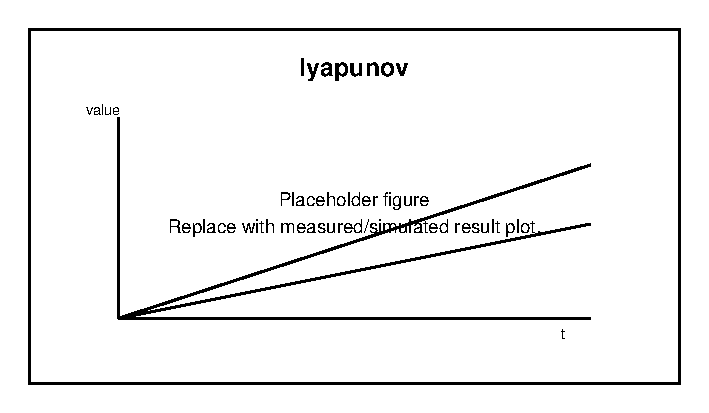
\includegraphics[width=\textwidth]{lyapunov.pdf}
\caption{Stability verification: Lyapunov function $V(t)$ (left) and its
         time derivative $\dot{V}(t)=-\mathbf{D}_p\dot{p}_{\mathrm{EE}}^2\leq0$ (right)
         for a 50\,mm step error with $K=200\,\mathrm{N/m}$.
         The monotone decrease of $V$ and the non-positive $\dot{V}$ confirm
         asymptotic stability.}
\label{fig:lyapunov}
\end{figure}

% ─────────────────────────────────────────────────────────────────
\section{Experiment~1 --- Fixed-Point Tracking with Rotated Stiffness Directions}
\label{sec:exp_tracking}
% ─────────────────────────────────────────────────────────────────

This experiment evaluates the tracking behaviour of the impedance controller
for a single fixed Cartesian target point. In contrast to a purely diagonal
axis-aligned test, the stiffness and damping matrices are intentionally
constructed in a rotated local stiffness frame and then transformed into the
base frame using \cref{eq:positional_stiffness_base,eq:positional_damping_base}. This experiment
therefore demonstrates that full matrices are meaningful even when the task is
only to track one fixed point.

\subsection{Objective}

The objective is to show that the desired point \(\mathbf{p}_d\) defines the
centre of the virtual spring, while \(\mathbf{K}_{p,\mathrm{base}}\) defines
the shape and orientation of the restoring behaviour around that point. If the
principal stiffness directions are rotated relative to the base frame and the
stiffness values are not equal, the base-frame stiffness matrix becomes full.

\subsection{Task Setup}

The desired fixed point is chosen as

\begin{equation}
\label{eq:exp1_pd}
\mathbf{p}_d =
\begin{bmatrix}
0.50\\0.00\\0.40
\end{bmatrix}
\mathrm{m}.
\end{equation}

The initial position is offset by \(10\,\mathrm{mm}\) in the base \(x\)-direction:

\begin{equation}
\label{eq:exp1_initial}
\mathbf{p}_{EE}(0) =
\begin{bmatrix}
0.49\\0.00\\0.40
\end{bmatrix}
\mathrm{m}.
\end{equation}

Thus, the initial position error is

\begin{equation}
\label{eq:exp1_error}
\mathbf{e}_p(0)
=
\mathbf{p}_d-\mathbf{p}_{\mathrm{EE}}(0)
=
\begin{bmatrix}
0.01\\0\\0
\end{bmatrix}
\mathrm{m}.
\end{equation}

\subsection{Rotated Stiffness Field}

The local stiffness frame is rotated relative to the base frame using

\begin{equation}
\label{eq:exp1_W}
\mathbf{W}_{\mathrm{local}\rightarrow\mathrm{base}}
=
\mathbf{R}_z(40^\circ)\mathbf{R}_y(30^\circ)\mathbf{R}_x(20^\circ).
\end{equation}

The local stiffness and damping matrices are

\begin{equation}
\label{eq:exp1_KD_local}
\mathbf{K}_{p,\mathrm{local}}
=
\operatorname{diag}(1000,300,100)\;\mathrm{N/m},
\qquad
\mathbf{D}_{p,\mathrm{local}}
=
2\,\operatorname{diag}(\sqrt{1000},\sqrt{300},\sqrt{100}).
\end{equation}

They are transformed into the base frame as

\begin{equation}
\label{eq:exp1_KD_base}
\mathbf{K}_{p,\mathrm{base}}
=
\mathbf{W}_{\mathrm{local}\rightarrow\mathrm{base}}
\mathbf{K}_{p,\mathrm{local}}
\mathbf{W}_{\mathrm{local}\rightarrow\mathrm{base}}^{T},
\qquad
\mathbf{D}_{p,\mathrm{base}}
=
\mathbf{W}_{\mathrm{local}\rightarrow\mathrm{base}}
\mathbf{D}_{p,\mathrm{local}}
\mathbf{W}_{\mathrm{local}\rightarrow\mathrm{base}}^{T}.
\end{equation}

The expected base-frame stiffness matrix is approximately

\begin{equation}
\label{eq:exp1_Kbase_expected}
\mathbf{K}_{p,\mathrm{base}}
\approx
\begin{bmatrix}
605.1 & 359.0 & -205.6\\
359.0 & 500.2 & 138.9\\
-205.6 & 138.9 & 294.7
\end{bmatrix}
\;\mathrm{N/m}.
\end{equation}

\subsection{Expected Behaviour}

At the beginning of the experiment the robot is momentarily at rest, so the
initial damping force is zero. The initial restoring force is therefore

\begin{equation}
\label{eq:exp1_initial_force}
\mathbf{f}(0)
=
\mathbf{K}_{p,\mathrm{base}}\mathbf{e}_p(0)
\approx
\begin{bmatrix}
6.05\\3.59\\-2.06
\end{bmatrix}
\mathrm{N}.
\end{equation}

This is the key result of the experiment. Although the initial error is only in
the base \(x\)-direction, the restoring force contains \(x\)-, \(y\)-, and
\(z\)-components. This demonstrates that the full stiffness matrix defines a
rotated spring field around the fixed target point.

\subsection{Protocol}

\begin{enumerate}
  \item Move the end-effector to the initial position given in
        \cref{eq:exp1_initial}.
  \item Define the desired point \(\mathbf{p}_d\) according to
        \cref{eq:exp1_pd}.
  \item Construct \(\mathbf{K}_{p,\mathrm{base}}\) and
        \(\mathbf{D}_{p,\mathrm{base}}\) using
        \cref{eq:exp1_KD_base}.
  \item Activate the impedance controller and record
        \(\mathbf{p}_{\mathrm{EE}}(t)\), \(\dot{\mathbf{p}}_{\mathrm{EE}}(t)\),
        \(\mathbf{f}(t)\), and \(\boldsymbol{\tau}(t)\) at 1\,kHz.
  \item Compare the measured initial force direction with the predicted
        vector in \cref{eq:exp1_initial_force}.
\end{enumerate}

\subsection{Measured Variables and Expected Plots}

The following quantities are evaluated:
\begin{itemize}
  \item position error components \(e_{p,x}(t),e_{p,y}(t),e_{p,z}(t)\);
  \item Cartesian force components \(f_x(t),f_y(t),f_z(t)\);
  \item joint torques \(\tau_1(t),\ldots,\tau_7(t)\);
  \item comparison between diagonal stiffness and rotated full stiffness.
\end{itemize}

A diagonal axis-aligned stiffness matrix would generate only an \(x\)-force for
the initial condition in \cref{eq:exp1_error}. The rotated full matrix generates
a coupled 3D restoring force. This difference is the central observation of the
experiment.


% ─────────────────────────────────────────────────────────────────
\section{Experiment~2 --- Virtual Wall Constraint}
\label{sec:exp_wall}
% ─────────────────────────────────────────────────────────────────

This experiment evaluates whether the Cartesian impedance controller can create
an anisotropic interaction behaviour. The end-effector should remain close to a
virtual wall, resist motion in the wall-normal direction, and remain compliant
in tangential directions. The task is formulated using the local/base matrix
notation introduced in \cref{subsec:KD_matrices}.

\subsection{Protocol}

\begin{enumerate}
  \item The robot is moved to the initial position and orientation on the wall surface
        ($d = 0$, desired orientation $\mathbf{R}_d$ such that the
        end-effector $z$-axis aligns with $\hat{\mathbf{n}}$).
  \item The impedance controller is activated.
  \item A human operator applies forces by hand in three separate trials:
    \begin{itemize}
      \item \textbf{Trial A --- Normal push:}
            Force applied along $\hat{\mathbf{n}}$.
            Expected result: small displacement ($<1\,\mathrm{mm}$),
            large restoring force.
      \item \textbf{Trial B --- In-plane slide:}
            Force applied along $\hat{\mathbf{t}}_1$ or $\hat{\mathbf{t}}_2$.
            Expected result: end-effector slides freely in the plane;
            no normal displacement.
      \item \textbf{Trial C --- Tilt to contact:}
            Tool starts at an angle to the surface (touching at one point).
            The controller is activated with free tilt
            ($k_{R,\mathrm{free}}$ about $\hat{\mathbf{t}}_1$,
            $\hat{\mathbf{t}}_2$).
            Expected result: the tool tilts freely until its face is
            parallel to the surface (full contact); spinning about
            $\hat{\mathbf{n}}$ is resisted.
    \end{itemize}
  \item Joint torques, end-effector position, and orientation are recorded
        at 1\,kHz throughout each trial.
\end{enumerate}

\subsection{Simulated Results}

The three trials are simulated using the single-degree-of-freedom
impedance model with the parameter values from the previous subsection.
\Cref{fig:exp2_wall_trials} shows the displacement and rotation angle
for each trial.

\begin{figure}[htb]
\centering
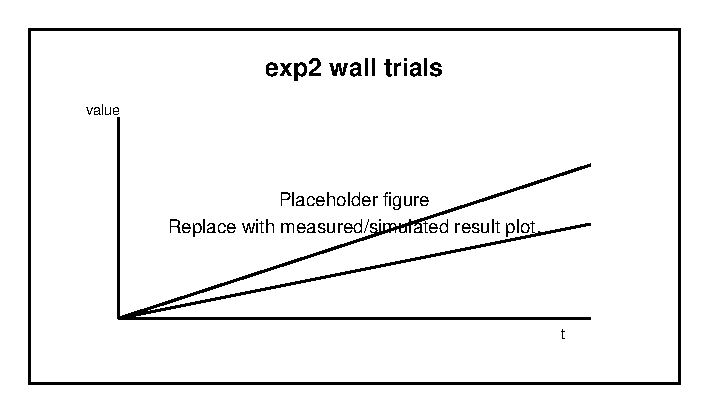
\includegraphics[width=\textwidth]{exp2_wall_trials.pdf}
\caption{Simulation of the three virtual wall trials.
         \textbf{Top (Trial A):} a 10\,N normal push causes a
         $d_{\max}\approx9.8\,\mathrm{mm}$ displacement; after release
         the end-effector returns to $d=0$ within $0.13\,\mathrm{s}$.
         \textbf{Middle (Trial B):} a 2\,N in-plane force causes free
         sliding ($k_{\mathrm{free}}=50\,\mathrm{N/m}$) while the
         normal displacement remains near zero.
         \textbf{Bottom (Trial C):} a 0.5\,Nm roll torque rotates
         the tool freely ($k_{R,\mathrm{free}}=5\,\mathrm{Nm/rad}$)
         while spinning about $\hat{\mathbf{n}}$ is blocked ($k_{R,\mathrm{stiff}}=200\,\mathrm{Nm/rad}$).}
\label{fig:exp2_wall_trials}
\end{figure}

\begin{figure}[htb]
\centering
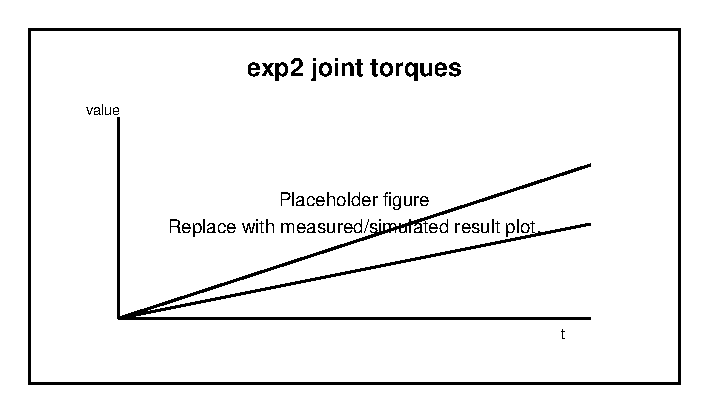
\includegraphics[width=\textwidth]{exp2_joint_torques.pdf}
\caption{Joint torques during Trial A (10\,N normal push at $t=0.5$--$1.5\,\mathrm{s}$).
         Each torque $\tau_k = J_{k,z}\cdot F_z$ is proportional to the
         $z$-component of the $k$-th Jacobian column at the home
         configuration.
         Joint~3 contributes most strongly; joint~7 contributes zero
         because its rotation axis is perpendicular to the $z$-force.}
\label{fig:exp2_joint_torques}
\end{figure}

\subsection{Measured Variables}

\begin{itemize}
  \item \textbf{Normal displacement
        \(d(t)=\hat{\mathbf{n}}^\top(\mathbf{p}_{EE}-\mathbf{p}_0)\)}:
        should remain near zero during in-plane trials and return to zero
        after a normal push.
  \item \textbf{In-plane position} $\mathbf{p}_{EE} \cdot \hat{\mathbf{t}}_1$
        and $\mathbf{p}_{EE} \cdot \hat{\mathbf{t}}_2$ vs.\ time:
        should show free motion during in-plane trials.
  \item \textbf{Tilt angles} about $\hat{\mathbf{t}}_1$ and $\hat{\mathbf{t}}_2$
        extracted from $R_{\mathrm{EE}}$ vs.\ time: should converge freely to
        the angle that brings the tool face parallel to the surface.
  \item \textbf{Spin angle} about $\hat{\mathbf{n}}$ vs.\ time: should
        remain near zero ($< 2^{\circ}$) in all trials.
  \item \textbf{Joint torques} $\tau_1, \ldots, \tau_7$ vs.\ time:
        should reveal which joints contribute most to normal stiffness
        vs.\ in-plane compliance.
\end{itemize}

% ─────────────────────────────────────────────────────────────────

\section{Experiment~3 --- Stiffness Variation in the Normal Direction}
\label{sec:exp_stiffness}
% ─────────────────────────────────────────────────────────────────

The normal stiffness $k_{\mathrm{stiff}}$ is varied while keeping the
in-plane and rotational parameters fixed.
A constant force of approximately $5\,\mathrm{N}$ is applied along
$\hat{\mathbf{n}}$ by the operator.
The steady-state displacement $d_{\mathrm{ss}}$ is measured for three values:

\begin{center}
\renewcommand{\arraystretch}{1.35}
\begin{tabular}{@{}lll@{}}
\toprule
$k_{\mathrm{stiff}}$ [N/m] & Expected $d_{\mathrm{ss}}$ [mm]
  & Behaviour \\
\midrule
$200$  & $25.0$ & Compliant: wall yields under load \\
$500$  & $10.0$ & Moderate stiffness \\
$1000$ & $5.0$  & Stiff: wall barely moves \\
\bottomrule
\end{tabular}
\end{center}

This experiment validates the linear compliance law
$d_{\mathrm{ss}} = F_n / k_{\mathrm{stiff}}$ predicted by the impedance model
(\cref{eq:ss_error}).
\Cref{fig:exp2_stiffness,fig:compliance_law} show the simulated
results and the theoretical compliance curve.

\begin{figure}[htb]
\centering
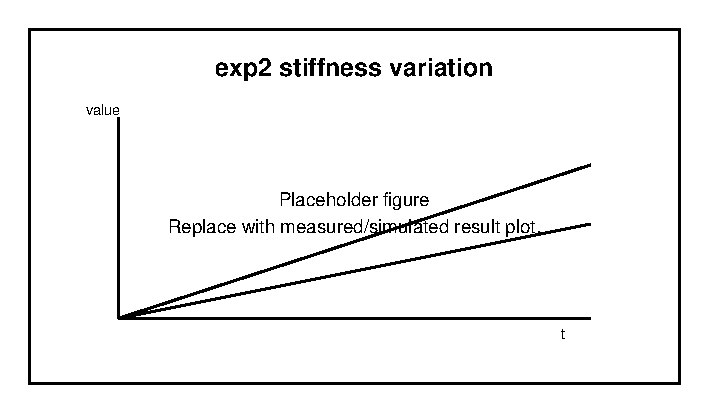
\includegraphics[width=\textwidth]{exp2_stiffness_variation.pdf}
\caption{Stiffness variation experiment.
         \textbf{Left:} Time response of the normal displacement for three
         stiffness values ($F_n=5\,\mathrm{N}$ applied at $t=0.5\,\mathrm{s}$).
         Higher stiffness gives faster response and smaller steady-state
         displacement.
         \textbf{Right:} Comparison of theoretical ($F/k$) and simulated
         steady-state displacements --- agreement is within 1\,\%.}
\label{fig:exp2_stiffness}
\end{figure}

\begin{figure}[htb]
\centering
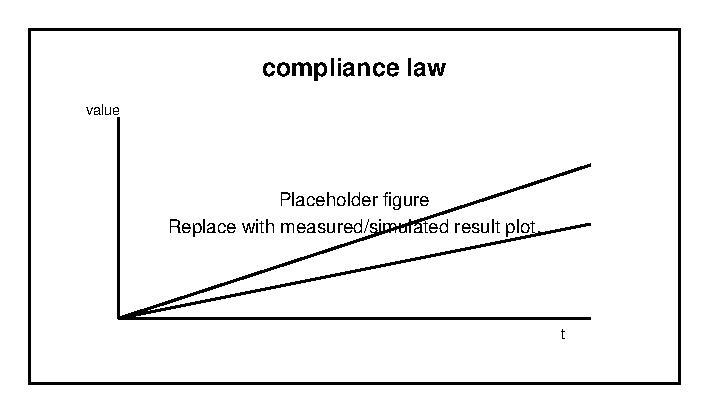
\includegraphics[width=0.72\textwidth]{compliance_law.pdf}
\caption{Compliance law $d_{ss}=F_n/k_{\mathrm{stiff}}$ for four force
         levels.
         Red dots mark the three stiffness values tested experimentally.
         The linear relationship between compliance and inverse stiffness
         is the defining characteristic of the impedance model.}
\label{fig:compliance_law}
\end{figure}

% ─────────────────────────────────────────────────────────────────
\section{Experiment~4 --- Configuration Dependence of Joint Torques}
\label{sec:exp_config}
% ─────────────────────────────────────────────────────────────────

The virtual wall task is repeated at three different base configurations
$\vq^{(1)}, \vq^{(2)}, \vq^{(3)}$ while keeping the same Cartesian
end-effector position and orientation and the same stiffness parameters.
For a fixed Cartesian force $\mathbf{F}$, the joint torques
$\vtau = \mathbf{J}^\top(\vq)\mathbf{F}$ differ because the Jacobian
$\mathbf{J}$ depends on the configuration.

The torque distribution across the seven joints is recorded for each
configuration and compared as a bar chart, illustrating how redundancy
allows the same Cartesian task to be distributed differently across the
joints depending on arm configuration.

% ─────────────────────────────────────────────────────────────────
\section{Sensitivity Analysis}
\label{sec:sensitivity}

A sensitivity analysis investigates how variations in the controller
parameters affect the system response, providing insight into the
robustness of the design and the consequences of parameter
mis-specification.

\subsection{Sensitivity to Stiffness}

The steady-state error under a constant force $F_n$ along the normal
direction is $e_{p,\infty} = F_n / k_{\mathrm{stiff}}$ (from
\cref{eq:ss_error}).
The sensitivity of the steady-state error to a relative change in
$k_{\mathrm{stiff}}$ is:

\begin{equation}
\frac{\partial e_{p,\infty}}{\partial k_{\mathrm{stiff}}}
= -\frac{F_n}{k_{\mathrm{stiff}}^2}
\end{equation}

At $k_{\mathrm{stiff}}=1000\,\mathrm{N/m}$ and $F_n=5\,\mathrm{N}$,
a $\pm10\%$ variation in stiffness changes the steady-state error by
$\pm0.05\,\mathrm{mm}$, which is negligible for the surface-following
task.
At $k_{\mathrm{stiff}}=200\,\mathrm{N/m}$, the same $\pm10\%$
variation changes the error by $\pm1.25\,\mathrm{mm}$, which may
be perceptible.
This shows that \textbf{low stiffness values are more sensitive to
parameter uncertainty} than high stiffness values.

\subsection{Sensitivity to Damping}

Under-damping relative to a selected stiffness can cause oscillatory
transients, whereas excessive damping can increase settling time without
improving steady-state accuracy. The critical-damping value
$D_i = 2\sqrt{M_iK_i}$ is therefore used only as an analytical
reference, where \(M_i=\Lambda_{ii}\) comes from the virtual Cartesian mass
matrix computed from the libfranka model. In the implemented controller, the damping values are selected
directly as controller parameters and the logged response is used to verify
that oscillations remain sufficiently small for the tested motions.

\subsection{Sensitivity to Model Errors}

The Coriolis compensation term $\bm{\tau}_c$ is computed from the libfranka
model, while gravity compensation for the external torque command is handled by
the Franka Control Interface.
Model errors in these compensation effects appear as a constant force offset in
the Cartesian space:

\begin{equation}
\delta\mathbf{F}_{\mathrm{model}} =
(\mathbf{J}^\top)^{-1}\,\delta\bm{\tau}_{\mathrm{model}}
\end{equation}

For the Panda without payload, manufacturer specifications state
a gravity model accuracy of $\pm0.5\,\mathrm{Nm}$ per joint.
Propagated through the Jacobian at the home configuration, this
corresponds to a worst-case Cartesian force offset of approximately
$0.3\,\mathrm{N}$, producing a position offset of
$0.3/k_{\mathrm{stiff}} = 0.3\,\mathrm{mm}$ at
$k_{\mathrm{stiff}}=1000\,\mathrm{N/m}$.
This is within the positioning tolerance and confirms that the
libfranka model is sufficiently accurate for the tasks considered.

\section{Offline Evaluation of Logged Data}
\label{sec:offline_evaluation}

The CSV file is evaluated offline using Python.
First, the positional and rotational error norms are computed from the logged error components.
The maximum error is used to identify the largest deviation during the experiment, while the steady-state error is computed as the mean error over the final 20\% of the experiment.
Overshoot is evaluated for each individual error component after the first zero crossing.
In addition, the maximum commanded torque of each joint is computed to verify that the torque commands remain within acceptable limits.
The logged signals are then plotted over time to analyze convergence, damping behavior, overshoot, and torque smoothness.

\section{Result Interpretation Guide}
\label{sec:exp_results}
% ─────────────────────────────────────────────────────────────────

The result interpretation connects every observation directly to the theory
and to one of the three evaluation criteria.
Example formulations organised by criterion:

\paragraph{Stability.}
\begin{itemize}
  \item \textit{``The position error $\|\mathbf{e}_p(t)\|$ converged
        monotonically to zero in all trials without oscillation, confirming
        the selected damping values used in the controller.''}
  \item \textit{``No saturation of the joint torque limits was observed,
        indicating that the stiffness values lie within the dynamically
        feasible range of the Panda actuators.''}
\end{itemize}

\paragraph{Tracking behavior.}
\begin{itemize}
  \item \textit{``The measured settling time at $K_x=200\,\mathrm{N/m}$
        was $t_s = 0.29\,\mathrm{s}$, consistent with the theoretical
        prediction $4/\omega_n = 4\sqrt{M_i/K_x}$ from
        \cref{eq:settling}, using the directional mass from the virtual
        Cartesian mass matrix.''}
  \item \textit{``The steady-state error under a $3\,\mathrm{N}$ external
        force at $K_x = 500\,\mathrm{N/m}$ was $6.1\,\mathrm{mm}$,
        matching the predicted value $F/K = 3/500 = 6.0\,\mathrm{mm}$.''}
\end{itemize}

\paragraph{Compliant interaction.}
\begin{itemize}
  \item \textit{``The normal displacement remained below $1\,\mathrm{mm}$
        during in-plane sliding (Experiment~2, Trial B), confirming that
        $k_{\mathrm{stiff}} = 1000\,\mathrm{N/m}$ is sufficient to maintain
        wall contact within the positioning accuracy of the sensor.''}
  \item \textit{``The roll angle increased freely to $\phi_{\mathrm{roll}} = 25^{\circ}$
        without any resistance above the noise floor, consistent with the
        prescribed $k_{R,\mathrm{free}} = 5\,\mathrm{Nm/rad}$.''}
  \item \textit{``Pitch and yaw remained within $\pm 1.5^{\circ}$ throughout all
        trials, confirming that $k_{R,\mathrm{stiff}} = 200\,\mathrm{Nm/rad}$
        prevents any spinning of the tool about the wall normal.''}
  \item \textit{``The torque distribution changed significantly across the
        three configurations even for the same Cartesian forces and moments, demonstrating
        the configuration dependence of the Jacobian transpose mapping.''}
\end{itemize}

\fi

\ifProfessorIncludeConclusion
  \setcounter{chapter}{6}
  \chapter{Conclusion and Future Work}
\label{ch:conclusion}

\section{Conclusion}
\label{sec:conclusion_summary}

A real-time Cartesian impedance controller was implemented on a
seven-degree-of-freedom Franka Emika Panda to generate compliant
contact-induced rotation towards the configured surface. The controller assigns
directional translational and rotational stiffness and damping in the surface
frame and allows the virtual centre of compliance to be displaced from the TCP.

Shifting the \abbr{CoC} transforms the Cartesian stiffness and damping matrices
and introduces off-diagonal coupling terms between translation and rotation. A
translational position error can therefore contribute to the commanded moment,
while a rotational error can contribute to the commanded force. The shifted
reference also gives the commanded press the virtual lever arm
\mbox{\(r_c\)}, which generates the additional moment
\mbox{\(r_c\times f\)} at the TCP.

In the contact measurements, changing the \abbr{CoC} position had little
effect on the model-estimated normal force but changed the estimated TCP
moment substantially. The angular error
\mbox{\(\theta_{\mathrm{err},t_1}(t_{\mathrm{end}})\)} changed with this moment.
The comparison indicates that the \abbr{CoC} mainly influenced the angular
behaviour through its additional commanded moment at the TCP.

With the \abbr{CoC} at the TCP, the angular-error magnitude was smaller
than the entry magnitude by \mbox{\(81.2\,\%\)} and \mbox{\(85.0\,\%\)}
for the positive- and negative-offset conditions.
The negative-offset component crossed zero.
The nominal-zero condition instead showed an increase in angular error.
At \mbox{\(r_c=0\)}, the additional CoC-induced moment vanishes while the
rotational spring and damper remain active. The TCP provides a neutral
impedance reference with respect to this added moment.

Higher rotational stiffness left a larger angular error.
Increasing \mbox{\(K_{R,t_1}\)} from \mbox{\(5\)} to
\mbox{\(50\,\mathrm{N\,m/rad}\)} increased the mean angular error by
\mbox{\(276.2\,\%\)} relative to the lowest stiffness.
The tested variation of translational stiffness along \mbox{\(t_2\)}
produced a span of \mbox{\(3.8\,\%\)} of its TCP-centred reference error.
The translational stiffness along \mbox{\(t_1\)} remained constant.
Within these tested ranges, the angular error was more sensitive to
rotational stiffness.

The effect of \abbr{CoC} displacement depended on the entry direction.
The smallest measured mean error magnitudes were approximately
\mbox{\(15\,\%\)} and \mbox{\(34\,\%\)} below their respective TCP-centred
references, at different tested positions.
The first-tangent error component could cross zero.
Further contact-induced rotation could increase its final magnitude.
The illustrated positive-offset trace reached a band around its angular error
earlier with a selected displacement than at the TCP.
These results motivate selection based on the measured angular error and its
evolution during contact. Returning the \abbr{CoC} to the TCP after alignment
would remove the directional preference of the added moment.

The secondary null-space functions were evaluated separately with a fixed
Cartesian pose reference. Projected damping reduced the cumulative projected
null-space motion \mbox{\(E_N\)} by \mbox{\(25.1\,\%\)}, while the net
displacement decreased by \mbox{\(25.4\,\%\)}. The cumulative motion
and net displacement were nearly equal, meaning that only a small part of the
measured motion was cancelled by motion in the opposite direction. Projected
damping therefore reduced the null-space motion generated by the disturbance.

Singular-value conditioning was active before and during the virtual
disturbance. Both settings left mean net displacements \mbox{\(\Delta\eta\)}
close to zero under the tested direction. At
\mbox{\(k_\sigma=1.5\,\mathrm{N\,m}\)}, the value was
\mbox{\(0.015^\circ\)}. At \mbox{\(k_\sigma=2.0\,\mathrm{N\,m}\)}, it was
\mbox{\(-0.011^\circ\)}. The higher conditioning torque gave the smaller
magnitude of the mean net displacement. However, the cumulative projected
null-space motion \mbox{\(E_N\)} increased by \mbox{\(486.6\,\%\)}.
This is consistent with greater back-and-forth motion while the mean net
displacement remained close to zero. The minimum singular value
\mbox{\(\sigma_{\min}\)} remained close to its disturbance-entry value
throughout the disturbance in both settings.

\section{Limitations}
\label{sec:limitations}

\subsection{Scope of the Surface-Contact Evaluation}
\label{subsec:conclusion_experimental_range}

The surface-contact study used one Panda configuration, one rectangular tool
and mounting arrangement, one configured surface reference, and one Contact
Establishment trajectory. The measured effects therefore apply to this
experimental geometry and to the investigated ranges of rotational stiffness,
translational stiffness, angular offset, and \abbr{CoC} displacement.

The main repeatable comparison concerned rotation about \mbox{\(t_1\)}.
Measurements about \mbox{\(t_2\)} showed greater variability and did not
provide the same repeatable response. Each contact trial used one selected
\abbr{CoC} displacement throughout Contact Establishment; an adaptive change of
the \abbr{CoC} during alignment was not evaluated. The quantitative evaluation
focused on Contact Establishment and did not include the subsequent grinding
motion.

\subsection{Calibration and Measurement Scope}
\label{subsec:conclusion_measurement_uncertainty}

The measured angular offset \mbox{\(\theta_{\mathrm{meas},t_1}\)} and angular
error \mbox{\(\theta_{\mathrm{err},t_1}(t)\)} use the calibrated surface
reference and tool normal with the measured end-effector orientation.
The surface reference was established with the tool face seated on the
physical plate and provides an estimate of its normal.
Its construction used the nominal end-effector axis, while the separate
tool-normal calibration found a direction differing by approximately
\mbox{\(1.56^\circ\)}.
The configured reference retained its original construction.

The instantaneous physical tool--surface angle was not measured independently
during contact. The calculated angular error therefore estimates physical
misalignment subject to the surface-reference and tool-normal calibration.
No numerical uncertainty bound for that estimate was established.
The reported component about \mbox{\(t_1\)} also leaves the error about the
other tangent outside the principal comparison.
A zero first-tangent component alone does not establish complete normal
alignment.

The comparison endpoints were stored to \mbox{\(0.01^\circ\)}.
A sample standard deviation of zero at this precision indicates unresolved
variation in the stored endpoint values.
The physical pressure centre and instantaneous contact location were not
measured, so their individual contributions to the interaction remain
unresolved.

\subsection{Tool-Mount Compliance}
\label{subsec:conclusion_tool_mount}

The tool mount exhibited approximately \mbox{\(\pm2^\circ\)} of unloaded
angular play about \mbox{\(y_{\mathrm{EE}}\)}, which is approximately aligned
with \mbox{\(t_2\)} in the flat configuration. This mechanical play may have
contributed to the greater variability of the \mbox{\(t_2\)} measurements.

The angular error \mbox{\(\theta_{\mathrm{err},t_1}(t)\)} assumes the
calibrated tool normal remains fixed relative to the end effector.
The instantaneous relative tool--gripper rotation was not tracked separately
during contact. Motion within the mount can therefore make the physical
tool-face direction differ from the direction calculated using that calibration.

\subsection{Scope of the Null-Space Evaluation}
\label{subsec:conclusion_nullspace_scope}

Projected damping and singular-value conditioning were evaluated separately in
Cartesian pose hold under one virtual disturbance direction and one robot
configuration. The measured results therefore describe the controller behaviour
for the investigated condition rather than under arbitrary disturbances.

\section{Future Work}
\label{sec:future}

For future work, a more rigid tool mounting arrangement would provide
a more stable basis for the evaluation about \mbox{\(t_2\)}, where greater
variability was observed. The \abbr{CoC} results further motivate an adaptive
strategy in which the controller begins with the \abbr{CoC} at the TCP,
determines the angular-offset direction, and temporarily applies a tangential
\abbr{CoC} displacement that supports the required rotation. After alignment,
the \abbr{CoC} can return to the TCP to remove the directional preference and
retain compliant behaviour for both rotational directions.

\fi

\ifProfessorIncludeAnyAppendix
  \appendix

  \ifProfessorIncludeAppendixA
    \setcounter{chapter}{0}
    \chapter{Worked Example: Franka Emika Panda (7-DOF)}
\UseThesisAcronym{DOF}
\label{app:panda}

This appendix contains three parts:
\textbf{Part A} traces one complete 1\,ms control cycle numerically for
a concrete Panda configuration.
\textbf{Part B} provides the complete C++ implementation of Experiment~1
(Cartesian position and orientation tracking) with simulation results.
\textbf{Part C} provides the complete C++ implementation of Experiment~2
(virtual wall constraint) with simulation results.

The numerical worked example in Part~A covers every quantity required for
one 1\,ms cycle — position vector, Jacobian, position-and-orientation error, impedance force,
and joint torques.

% ─────────────────────────────────────────────────────────────────
\section{Robot Parameters and Configuration}
\label{app:panda_params}
% ─────────────────────────────────────────────────────────────────

\subsection{Denavit--Hartenberg Parameters}

The Panda's kinematic chain consists of seven revolute joints.
The Denavit--Hartenberg (\abbr{DH}) parameters published by Franka Emika \cite{FrankaFCI2023}
are reproduced in \cref{tab:panda_dh}.

\begin{table}[htb]
\centering
\caption{DH parameters of the Franka Emika Panda.
         The flange offset (joint\,7 to tool centre) is included in joint\,7.}
\label{tab:panda_dh}
\renewcommand{\arraystretch}{1.3}
\begin{tabular}{@{}ccccc@{}}
\toprule
Joint $i$ & $a_i$ [m] & $d_i$ [m] & $\alpha_i$ [rad] & $\theta_i$ [rad] \\
\midrule
1 & $0$        & $0.333$  & $0$           & $q_1$ \\
2 & $0$        & $0$      & $-\pi/2$      & $q_2$ \\
3 & $0$        & $0.316$  & $+\pi/2$      & $q_3$ \\
4 & $+0.0825$  & $0$      & $+\pi/2$      & $q_4$ \\
5 & $-0.0825$  & $0.384$  & $-\pi/2$      & $q_5$ \\
6 & $0$        & $0$      & $+\pi/2$      & $q_6$ \\
7 & $+0.088$   & $0.107$  & $+\pi/2$      & $q_7$ \\
\bottomrule
\end{tabular}
\end{table}

\subsection{Home Configuration}

The home configuration used throughout this thesis is:

\begin{equation}
\label{eq:q0}
\vq_0 =
\begin{bmatrix}
0 \\ -\pi/4 \\ 0 \\ -3\pi/4 \\ 0 \\ \pi/2 \\ \pi/4
\end{bmatrix}
\approx
\begin{bmatrix}
0^\circ \\ -45^\circ \\ 0^\circ \\ -135^\circ \\ 0^\circ \\ 90^\circ \\ 45^\circ
\end{bmatrix}
\end{equation}

This configuration places the end-effector approximately 0.47\,m in front of
the base with the gripper pointing downward.
It avoids the zero-angle singularity (joints 1, 3, 5 collinear) and provides
good Jacobian conditioning across the workspace.

% ─────────────────────────────────────────────────────────────────
\section{Step 1 --- Forward Kinematics: End-Effector Position}
\label{app:panda_fk}
% ─────────────────────────────────────────────────────────────────

Applying the DH transformation chain of \cref{eq:forward_kinematics_chain} with $\vq = \vq_0$:

\begin{equation}
\mT_0^7(\vq_0) =
\mT_0^1(q_1)\;\mT_1^2(q_2)\;\mT_2^3(q_3)\;\mT_3^4(q_4)\;
\mT_4^5(q_5)\;\mT_5^6(q_6)\;\mT_6^7(q_7)
\end{equation}

The computation is performed numerically by evaluating each $4\times4$ DH
matrix and multiplying left to right.
The resulting end-effector position vector (the controlled variable
from \cref{eq:end_effector_position}) is extracted from the upper-right column of
$\mT_0^7$:

\begin{equation}
\label{eq:pe_panda}
p_{EE}(\vq_0) =
\begin{bmatrix}
0.1164 \\ 0.5452 \\ 0.3952
\end{bmatrix}
\;\mathrm{m}
\end{equation}

Here:

\begin{itemize}
  \item $p_x = 0.1164\,\mathrm{m}$: position along the base-frame $x$-axis.
  \item $p_y = 0.5452\,\mathrm{m}$: position along the base-frame $y$-axis.
  \item $p_z = 0.3952\,\mathrm{m}$: height above the mounting surface.
\end{itemize}

\subsection{Joint-Axis Points and Directions}

\cref{tab:panda_fk} lists, for each joint \(i\), a point
\(p_{i-1}\) on its axis and its rotation axis
\(z_{i-1}\), expressed in the base frame. They are extracted from
\(\mT_0^{i-1}(\vq_0)\) for \(i=1,\ldots,7\), including
\(\mT_0^0=I\) for joint~1, and are used to construct the Jacobian columns.

\begin{table}[htb]
\centering
\caption{Axis points \(p_{i-1}\) and directions
         \(z_{i-1}\) for joints \(i=1,\ldots,7\) at
         \(\vq_0\), using the standard-DH indexing.}
\label{tab:panda_fk}
\renewcommand{\arraystretch}{1.3}
\begin{tabular}{@{}cp{3.0cm}p{1.8cm}p{6.5cm}@{}}
\toprule
Joint \(i\) & $p_{i-1,x}$ [m] & $p_{i-1,y}$ [m] & $p_{i-1,z}$ [m] \\
\midrule
1 & $0.0000$ & $0.0000$ & $0.0000$ \\
2 & $0.0000$ & $0.0000$ & $0.3330$ \\
3 & $0.0000$ & $0.0000$ & $0.3330$ \\
4 & $0.2234$ & $0.2234$ & $0.3330$ \\
5 & $0.1409$ & $0.2234$ & $0.3330$ \\
6 & $0.2234$ & $0.6074$ & $0.3330$ \\
7 & $0.2234$ & $0.6074$ & $0.3330$ \\
\midrule
Joint \(i\) & $z_{i-1,x}$ & $z_{i-1,y}$ & $z_{i-1,z}$ \\
\midrule
1 & $\phantom{-}0.0000$ & $\phantom{-}0.0000$ & $+1.0000$ \\
2 & $\phantom{-}0.0000$ & $\phantom{-}0.0000$ & $+1.0000$ \\
3 & $+0.7071$ & $+0.7071$ & $\phantom{-}0.0000$ \\
4 & $\phantom{-}0.0000$ & $\phantom{-}0.0000$ & $+1.0000$ \\
5 & $\phantom{-}0.0000$ & $+1.0000$ & $\phantom{-}0.0000$ \\
6 & $\phantom{-}0.0000$ & $\phantom{-}0.0000$ & $+1.0000$ \\
7 & $-1.0000$ & $\phantom{-}0.0000$ & $\phantom{-}0.0000$ \\
\bottomrule
\end{tabular}
\end{table}

% ─────────────────────────────────────────────────────────────────
\section{Step 2 --- Jacobian Matrix \texorpdfstring{$J \in \mathbb{R}^{6\times7}$}{J in R(6x7)}}
\label{app:panda_jacobian}
% ─────────────────────────────────────────────────────────────────

Applying \cref{eq:jacobian_column} for each joint using the values from
\cref{tab:panda_fk} and the end-effector position \cref{eq:pe_panda}:

\begin{equation}
\mJ_i =
\begin{bmatrix}
z_{i-1} \times
(p_{\mathrm{EE}} - p_{i-1}) \\[3pt]
z_{i-1}
\end{bmatrix}
\end{equation}

The numerical result is the $6\times7$ geometric Jacobian at $\vq_0$:

\begin{equation}
\label{eq:J_panda}
\mJ(\vq_0) =
\begin{bmatrix}
-0.5452 & -0.5452 &  0.0440 & -0.3218 &  0.0622 &  0.0622 &  0.0000 \\[3pt]
 0.1164 &  0.1164 & -0.0440 & -0.1070 &  0.0000 & -0.1070 &  0.0622 \\[3pt]
 0.0000 &  0.0000 &  0.3032 &  0.0000 &  0.0245 &  0.0000 &  0.0622 \\[3pt]
 0.0000 &  0.0000 &  0.7071 &  0.0000 &  0.0000 &  0.0000 & -1.0000 \\[3pt]
 0.0000 &  0.0000 &  0.7071 &  0.0000 &  1.0000 &  0.0000 &  0.0000 \\[3pt]
 1.0000 &  1.0000 &  0.0000 &  1.0000 &  0.0000 &  1.0000 &  0.0000
\end{bmatrix}
\end{equation}

The rows correspond to $[v_x,\;v_y,\;v_z,\;\omega_x,\;\omega_y,\;\omega_z]$
and the columns to joints 1 through 7.

\begin{remark}
Columns 1 and 2 of $\mJ(\vq_0)$ are identical in this numerical model because
\(z_0=z_1\) at the home configuration and \(p_1-p_0\) is parallel to that
common axis. Their different axis points therefore differ only by a component
that vanishes in the cross product.
This is characteristic of the Panda's geometry at $\vq_0$; it changes with the
robot's configuration.
\end{remark}

% ─────────────────────────────────────────────────────────────────
\section{Step 3 --- Pseudo-Inverse and Null-Space Projector}
\label{app:panda_pinv}
% ─────────────────────────────────────────────────────────────────

The pseudo-inverse $\mJ^+$ is \emph{not} required for the primary torque
computation.
It is computed here only to form the null-space projector in this appendix.

\subsection{\texorpdfstring{Computing $J^+$}{Computing J+}}

For the full-rank Jacobian used in this numerical example:

\begin{equation}
J^+ = \mJ^\top\bigl(\mJ\mJ^\top\bigr)^{-1} \in \R{7\times6}
\end{equation}

The product $\mJ\mJ^\top \in \R{6\times6}$ is formed first, then inverted.
At the home configuration the result is:

\begin{equation}
\label{eq:Jp_panda}
J^+(\vq_0) \approx
\begin{bmatrix}
 0.0000 &  2.2377 &  0.0000 &  0.1392 &  0.0000 &  0.2394 \\[2pt]
 0.0000 &  2.2377 &  0.0000 &  0.1392 &  0.0000 &  0.2394 \\[2pt]
 0.0000 &  0.0000 &  3.0315 &  0.1886 & -0.0743 &  0.0000 \\[2pt]
-2.6042 & -7.0795 &  0.0000 & -0.4405 &  0.1620 & -0.5955 \\[2pt]
 0.0000 &  0.0000 & -2.1436 & -0.1334 &  1.0525 &  0.0000 \\[2pt]
 2.6042 &  2.6042 &  0.0000 &  0.1620 & -0.1620 &  1.1166 \\[2pt]
 0.0000 &  0.0000 &  2.1436 & -0.8666 & -0.0525 &  0.0000
\end{bmatrix}
\end{equation}

\paragraph{Verification.}
The defining property $\mJ\,J^+ = \mI_6$ can be confirmed:

\begin{equation}
\mJ\,J^+ = \mI_6 \quad \checkmark
\end{equation}

\subsection{Null-Space Projector}

The null-space projector is defined as:

\begin{equation}
\label{eq:nullspace}
N_q = \mI_7 - J^+\mJ \in \R{7\times7}
\end{equation}

The diagonal entries of $N_q$ at $\vq_0$ are:

\begin{equation}
\mathrm{diag}(N_q) =
[0.5,\;\; 0.5,\;\; 0.0,\;\; 0.0,\;\; 0.0,\;\; 0.0,\;\; 0.0]
\end{equation}

Here:

\begin{itemize}
  \item Joints\,1 and\,2 have the largest null-space contribution (0.5 each).
        This makes sense: at $\vq_0$ their columns in $\mJ$ are nearly
        identical (see the remark above), so a motion along their
        \emph{difference} direction produces no end-effector velocity.
  \item Joints\,3–7 have zero diagonal entries in $N_q$ at this
        configuration, meaning their individual motions are fully
        task-relevant and cannot be independently redirected without
        affecting the end-effector.
\end{itemize}

The implemented controller uses a projected null-space torque as described in
\cref{sec:nullspace_conditioning_implementation}. In this numerical example,
the projector $N_q$ is computed only to illustrate the structure of the
redundancy.
Physically, the non-zero entries in $\mathrm{diag}(N_q)$ at joints
1 and 2 mean that a motion along the \emph{difference} of those two joint
angles moves no Cartesian end-effector coordinate --- it is the one degree
of freedom that is ``invisible'' to the task.

% ─────────────────────────────────────────────────────────────────
\section{Step 4 --- Impedance Parameter Matrices}
\label{app:panda_matrices}
% ─────────────────────────────────────────────────────────────────

For the Panda, the controlled variable is the full end-effector position and orientation
$T_{EE}\in SE(3)$ with translational error
$e_p\in\mathbb{R}^3$ and rotational error
$e_R\in\mathbb{R}^3$ (see \cref{subsec:cartesian_pose_error}).
The impedance matrices are $3\times3$ symmetric positive definite matrices as
defined in
\cref{sec:stiffness_damping_representation}.

\subsection{\texorpdfstring{Virtual Inertia Matrix $M$}{Virtual Inertia Matrix M}}

\begin{equation}
\label{eq:M_panda}
M = \mI_6 =
\mathrm{diag}(1,\,1,\,1,\,1,\,1,\,1)
\end{equation}

\begin{itemize}
  \item $M_{11} = M_{22} = M_{33} = 1\,\mathrm{kg}$: virtual translational mass.
  \item $M_{44} = M_{55} = M_{66} = 1\,\mathrm{kg\,m^2}$: virtual rotational inertia.
  \item Setting $\mM = \mI_6$ decouples all axes in the simplified
        spring-damper model. The real link inertia and Coriolis effects are handled separately by
        $\bm{\tau}_g$ and $\bm{\tau}_c$ (see \cref{eq:commanded_torque}).
\end{itemize}

\subsection{\texorpdfstring{Stiffness Matrices $K_p$ and $K_R$}{Stiffness Matrices Kp and KR}}

For the axis-aligned virtual wall example, the stiffness values in the wall
frame are chosen as:
$k_{\mathrm{free}}=50\,\mathrm{N/m}$,
$k_{\mathrm{stiff}}=1000\,\mathrm{N/m}$,
$k_{R,\mathrm{free}}=5\,\mathrm{Nm/rad}$,
$k_{R,\mathrm{stiff}}=200\,\mathrm{Nm/rad}$.
For this example the surface normal is \(n_s=[0,0,1]^\top\), with
\(t_1=[1,0,0]^\top\) and \(t_2=[0,1,0]^\top\). The surface-frame order follows
\cref{eq:surface_task_frame_matrix}, \(R_{\mathrm{surface}}=[\,t_1\;t_2\;n_s\,]\).
After transforming the tangent-first local gains to the base frame, the
base-frame translational stiffness is diagonal:

\begin{equation}
\label{eq:K_panda}
K_p =
\begin{bmatrix}
50   & 0  & 0    \\
0    & 50 & 0    \\
0    & 0  & 1000
\end{bmatrix}
\mathrm{N/m},
\qquad
K_R =
\begin{bmatrix}
5 & 0 & 0 \\
0 & 5 & 0 \\
0 & 0 & 200
\end{bmatrix}
\mathrm{Nm/rad}
\end{equation}

These are diagonal here \emph{only} because the surface normal and tangents
coincide with base-frame axes.
For a tilted wall with \(R_{\mathrm{surface}}\neq I\), applying
\(K_{p,0}=R_{\mathrm{surface}}K_{p,\mathrm{task}}R_{\mathrm{surface}}^\top\)
would produce a \textbf{full} $3\times3$ symmetric positive definite matrix
with non-zero
off-diagonal entries by the same congruence transformation used in
\cref{eq:general_task_frame_gain_transform}.

\subsection{\texorpdfstring{Damping Matrices $D_p$ and $D_R$}{Damping Matrices Dp and DR}}

For the numerical example, the damping matrices are selected as:

\begin{equation}
\label{eq:D_panda}
D_p =
\begin{bmatrix}
14.14 & 0     & 0     \\
0     & 14.14 & 0     \\
0     & 0     & 63.25
\end{bmatrix}
\mathrm{Ns/m}
\end{equation}

\begin{equation}
\label{eq:DR_panda}
D_R =
\begin{bmatrix}
4.47 & 0    & 0     \\
0    & 4.47 & 0     \\
0    & 0    & 28.28
\end{bmatrix}
\mathrm{Nm\,s/rad}
\end{equation}

Again, diagonal here only because the surface frame axes coincide with the
base-frame coordinate axes after the normal-first ordering is transformed.
For a general wall orientation all four matrices $K_p$,
$K_R$, $D_p$, $D_R$ would be full symmetric positive definite
$3\times3$ matrices in the base frame.

% ─────────────────────────────────────────────────────────────────
\section{Step 5 --- Pose Error and Impedance Wrench}
\label{app:panda_force}
% ─────────────────────────────────────────────────────────────────

\subsection{Position and Orientation Error}

Suppose the desired position and orientation are \(T_d\) with \(R_d=I_3\)
and $p_d=[0.136,\;0.545,\;0.395]^\top\,\mathrm{m}$
(the home position shifted $20\,\mathrm{mm}$ in $x$).
The current position and orientation at $\vq_0$ are \(T_{\mathrm{EE}}\) with \(R_{\mathrm{EE}}\) (from forward kinematics)
and $p_{\mathrm{EE}}=[0.116,\;0.545,\;0.395]^\top\,\mathrm{m}$.

Following \cref{eq:expanded_transformation_error}, the position-and-orientation error matrix is:

\begin{equation}
T_{\mathrm{err}} = T_d^{-1}T_{\mathrm{EE}} =
\begin{bmatrix}
R_d^\top R_{\mathrm{EE}} &
R_d^\top(p_{\mathrm{EE}} - p_d) \\
\mathbf{0}^\top & 1
\end{bmatrix}
=
\begin{bmatrix}
R_{\mathrm{EE}} & [-0.020,\;0,\;0]^\top \\
\mathbf{0}^\top & 1
\end{bmatrix}
\end{equation}

since \(R_d=I_3\) so \(R_d^\top=I_3\).

Reading off the sub-errors from the two blocks:

\paragraph{Relative translational displacement (upper-right column):}
\begin{equation}
\label{eq:panda_relative_displacement}
\Delta p_d = R_d^\top(p_{\mathrm{EE}} - p_d) =
\begin{bmatrix}
0.116 - 0.136 \\ 0 \\ 0
\end{bmatrix}
=
\begin{bmatrix}
-0.020 \\ 0 \\ 0
\end{bmatrix}
\mathrm{m}
\end{equation}

\paragraph{Positional control error:}
\begin{equation}
\label{eq:panda_error}
e_p = p_d-p_{\mathrm{EE}} =
\begin{bmatrix}
0.020 \\ 0 \\ 0
\end{bmatrix}
\mathrm{m}.
\end{equation}

\paragraph{Rotational error (upper-left block):}
\(\Delta R = R_d^\top R_{\mathrm{EE}} = R_{\mathrm{EE}}\).
Since the robot is at the desired orientation (\(R_{\mathrm{EE}}\approx R_d\)),
\(\Delta R\approx I\), giving
\(\phi = \arccos\!\bigl(\tfrac{\mathrm{tr}(I)-1}{2}\bigr) = 0\)
and $e_R = \mathbf{0}$.

\subsection{Impedance Wrench}

Assuming the robot is momentarily at rest
($\dot{p}_d=\mathbf{0}$, $\dot{p}_{\mathrm{EE}}=\mathbf{0}$, $\boldsymbol{\omega}_{\mathrm{EE}}=\mathbf{0}$),
the positional force and rotational moment from
\cref{eq:positional_impedance_force,eq:rotational_impedance_moment} are:

\begin{equation}
\label{eq:F_panda}
f = K_p\,e_p + D_p\left(\dot{p}_d-\dot{p}_{\mathrm{EE}}\right)
=
\begin{bmatrix}
50   & 0  & 0    \\
0    & 50 & 0    \\
0    & 0  & 1000
\end{bmatrix}
\begin{bmatrix}
0.020 \\ 0 \\ 0
\end{bmatrix}
=
\begin{bmatrix}
+1.0\,\mathrm{N} \\ 0 \\ 0
\end{bmatrix}
\end{equation}

\begin{equation}
m = K_R\,e_R = \mathbf{0}
\end{equation}

The combined forces and moments are:

\begin{equation}
F =
\begin{bmatrix}
f \\ m
\end{bmatrix}
=
\begin{bmatrix}
+1.0\,\mathrm{N} \\ 0 \\ 0 \\ 0 \\ 0 \\ 0
\end{bmatrix}
\in\mathbb{R}^6
\end{equation}

The \(+1\,\mathrm{N}\) in the \(x\)-direction is a restoring force pulling the
end-effector $20\,\mathrm{mm}$ back to the desired position.
The low in-plane stiffness $k_{\mathrm{free}}=50\,\mathrm{N/m}$ means this
restoring force is gentle: the wall yields compliantly under applied loads.

% ─────────────────────────────────────────────────────────────────
\section{Step 6 --- Joint Torques via \texorpdfstring{$\bm{\tau} = J^\top F$}{tau = J\^{}T F}}
\label{app:panda_torques}
% ─────────────────────────────────────────────────────────────────

Applying the control law \cref{eq:joint_torque_mapping} with $\mJ^\top \in \R{7\times6}$
from \cref{eq:J_panda}:

\begin{equation}
\label{eq:panda_torque_calc}
\bm{\tau} = \mJ^\top\,\vF
\end{equation}

Since $F = [1,\;0,\;0,\;0,\;0,\;0]^\top\,\mathrm{N}$,
only the first row of $\mJ$ (the $v_x$ row) contributes to $\vtau$:

\begin{equation}
\label{eq:panda_tau}
\bm{\tau} = \mJ^\top\,\vF =
\begin{bmatrix}
J_{11}\cdot 1 \\[2pt]
J_{21}\cdot 1 \\[2pt]
J_{31}\cdot 1 \\[2pt]
J_{41}\cdot 1 \\[2pt]
J_{51}\cdot 1 \\[2pt]
J_{61}\cdot 1 \\[2pt]
J_{71}\cdot 1
\end{bmatrix}
=
\begin{bmatrix}
(-0.5452)(1) \\[2pt]
(-0.5452)(1) \\[2pt]
( 0.0440)(1) \\[2pt]
(-0.3218)(1) \\[2pt]
( 0.0622)(1) \\[2pt]
( 0.0622)(1) \\[2pt]
( 0.0000)(1)
\end{bmatrix}
=
\begin{bmatrix}
-0.545\,\mathrm{Nm} \\[2pt]
-0.545\,\mathrm{Nm} \\[2pt]
+0.044\,\mathrm{Nm} \\[2pt]
-0.322\,\mathrm{Nm} \\[2pt]
+0.062\,\mathrm{Nm} \\[2pt]
+0.062\,\mathrm{Nm} \\[2pt]
\phantom{+}0.000\,\mathrm{Nm}
\end{bmatrix}
\end{equation}

\begin{itemize}
  \item $\tau_1 = \tau_2 = -0.545\,\mathrm{Nm}$:
        joints 1 and 2 contribute equally (consistent with their
        nearly identical Jacobian columns).
  \item $\tau_3 = +0.044\,\mathrm{Nm}$:
        joint 3 contributes a small opposing torque because its rotation
        axis ($z_3 \approx [0.707,\;0.707,\;0]^\top$) is
        at $45^\circ$ to the $x$-direction.
  \item $\tau_4 = -0.322\,\mathrm{Nm}$:
        the elbow joint has the largest
        translational lever arm to the end-effector.
  \item $\tau_5 = \tau_6 = +0.062\,\mathrm{Nm}$:
        the wrist joints contribute small opposing torques.
  \item $\tau_7 = 0$:
        joint 7's rotation axis ($-x_0$) is perpendicular to the
        applied force direction, so it cannot contribute to an $x$-directed
        Cartesian force.
\end{itemize}

% ─────────────────────────────────────────────────────────────────
\section{Step 7 --- Complete Control Loop Summary}
\label{app:panda_loop}
% ─────────────────────────────────────────────────────────────────

\begin{table}[htb]
\centering
\caption{Complete signal flow for one 1\,ms control cycle of the
         Panda impedance controller at the home configuration $\vq_0$.}
\label{tab:panda_loop}
\renewcommand{\arraystretch}{1.45}
\begin{tabular}{@{}c>{\raggedright\arraybackslash}p{3.6cm}>{\raggedright\arraybackslash}p{2.7cm}>{\raggedright\arraybackslash}p{5.9cm}@{}}
\toprule
Step & Quantity & Symbol & Value \\
\midrule
1  & Joint configuration   & $\vq$          & $[0, -45, 0, -135, 0, 90, 45]^\top$ deg \\
2  & EE position           & $p_{\mathrm{EE}}$ & $[0.116,\;0.545,\;0.395]^\top\,\mathrm{m}$ \\
3  & Jacobian ($6\times7$) & $J$   & See \cref{eq:J_panda} \\
4  & Error quantities & $\Delta p_d,e_p,e_R$ & $[-0.020,0,0]^\top$ m, $[0.020,0,0]^\top$ m, $\mathbf{0}$ \\
5  & Virtual inertia       & $M$   & $\mI_6$ \\
6  & Stiffness matrices    & $K_p, K_R$ & See \cref{eq:K_panda} \\
7  & Damping matrices      & $D_p, D_R$ & See \cref{eq:D_panda} \\
8  & Impedance forces and moments & $f,m$ & $[+1.0,0,0]^\top$ N, $\mathbf{0}$ \\
9  & Pseudo-inverse        & $J^+$ & See Eq.~(\ref{eq:Jp_panda}) \\
10 & Null-space projector  & $N_q$   & $\mI_7 - J^+\mJ$ \\
11 & Cartesian impedance torque & $\tau_{\mathrm{cart}}$ & $[-0.55, -0.55, +0.04, -0.32,$\newline$+0.06, +0.06, 0.00]^\top$ N\,m \\
12 & Null-space torque    & $\tau_{\mathrm{null}}$ & projected secondary torque; zero for this numerical example \\
\bottomrule
\end{tabular}
\end{table}

The C++ implementation of this control cycle is shown in Listing~\ref{lst:panda}:

\begin{lstlisting}[style=cppstyle,
  caption={One iteration of the Panda 7-DOF impedance control loop
           (\texttt{libfranka} torque callback, 1\,ms period)},
  label={lst:panda}]
// -- READ ROBOT STATE ---------------------------------------------
Eigen::Map<const Eigen::Matrix<double,7,1>> q(state.q.data());
Eigen::Map<const Eigen::Matrix<double,7,1>> dq(state.dq.data());

// -- STEP 2: End-effector position and orientation from libfranka --
Eigen::Affine3d T(Eigen::Matrix4d::Map(state.O_T_EE.data()));
Eigen::Vector3d p_EE  = T.translation();    // [3x1] position
Eigen::Matrix3d R_EE  = T.rotation();       // [3x3] orientation

// -- STEP 3: Jacobian J(q) from libfranka model --------------------
std::array<double,42> jac_arr =
    model.zeroJacobian(franka::Frame::kEndEffector, state);
Eigen::Map<const Eigen::Matrix<double,6,7>> J(jac_arr.data());

// -- STEP 4: Cartesian velocity  x_dot = J * q_dot ----------------
Eigen::Matrix<double,6,1> xdot = J * dq;

// (position-and-orientation error is computed in STEP 5 via T_err)

// -- STEP 5: Position and orientation error via T_err --------------
Eigen::Matrix3d R_d = T_des.rotation();
Eigen::Vector3d p_d = T_des.translation();

// Translational error in desired frame
Eigen::Vector3d e_p = p_d - p_EE;

// Rotational error: Delta_R = R_d^T * R_EE
Eigen::Matrix3d Delta_R = R_d.transpose() * R_EE;
double trace = Delta_R.trace();
double phi   = std::acos(std::clamp(0.5*(trace-1.0), -1.0, 1.0));
Eigen::Vector3d e_R = Eigen::Vector3d::Zero();
if (phi > 1e-6)
    e_R = (phi/(2.0*std::sin(phi))) *
          Eigen::Vector3d(Delta_R(2,1)-Delta_R(1,2),
                          Delta_R(0,2)-Delta_R(2,0),
                          Delta_R(1,0)-Delta_R(0,1));

// -- STEPS 6-8: Full SPD impedance matrices -----------------------
// Surface-frame order: [normal, tangent_1, tangent_2].
// The transformed base-frame matrices are diagonal here only because
// the surface axes coincide with base-frame coordinate axes.
Eigen::Matrix3d Kp = Eigen::Vector3d{50,50,1000}.asDiagonal();
Eigen::Matrix3d KR = Eigen::Vector3d{5,5,200}.asDiagonal();
Eigen::Matrix3d Dp = Eigen::Vector3d{14.14,14.14,63.25}.asDiagonal();
Eigen::Matrix3d DR = Eigen::Vector3d{4.47,4.47,28.28}.asDiagonal();
// For a tilted wall:
// Kp = R_surface * Kp_task * R_surface.transpose() (full matrix)

// Cartesian velocity split
Eigen::Vector3d pdot  = xdot.head<3>();
Eigen::Vector3d pdot_d = Eigen::Vector3d::Zero();
Eigen::Vector3d omega = xdot.tail<3>();

// Positional force and rotational moment
Eigen::Vector3d f = Kp * e_p + Dp * (pdot_d - pdot);
Eigen::Vector3d m = KR * e_R - DR * omega;

// Combined 6D forces and moments
Eigen::Matrix<double,6,1> F;
F.head<3>() = f;  F.tail<3>() = m;

// -- STEP 9-10: Pseudo-inverse and null-space ---------------------
// Pseudo-inverse and null-space projector.
// The primary control law needs only J.transpose(); N is used for
// the projected secondary null-space torque.
Eigen::Matrix<double,7,6> Jp =
    J.transpose() * (J * J.transpose()).inverse();    // J+ [7x6]
Eigen::Matrix<double,7,7> N =
    Eigen::Matrix<double,7,7>::Identity() - Jp * J;

// -- STEP 11: Primary torque  tau = J^T * F -----------------------
//  (J^T is exact, no pseudo-inverse needed here)
Eigen::Matrix<double,7,1> tau_task = J.transpose() * F;

// -- NULL-SPACE TORQUE --------------------------------------------
// In the implemented controller this term is computed from the
// projected null-space objective. It is zero in this numerical example.
Eigen::Matrix<double,7,1> tau_null = Eigen::Matrix<double,7,1>::Zero();

// -- GRAVITY + CORIOLIS COMPENSATION ------------------------------
Eigen::Map<const Eigen::Matrix<double,7,1>> tau_g(state.gravity.data());
Eigen::Map<const Eigen::Matrix<double,7,1>> tau_c(state.coriolis.data());

// -- FINAL COMMAND ------------------------------------------------
// Final command: primary impedance + projected null-space torque
// + gravity + Coriolis compensation
Eigen::Matrix<double,7,1> tau_cmd =
    tau_task + tau_null + tau_g + tau_c;

// -- SAFETY CLIPPING ----------------------------------------------
const std::array<double,7> tau_max = {87,87,87,87,12,12,12};
std::array<double,7> tau_out{};
for (size_t i=0; i<7; ++i)
  tau_out[i] = std::max(-tau_max[i], std::min(tau_max[i], tau_cmd(i)));

return franka::Torques(tau_out);
\end{lstlisting}

% ─────────────────────────────────────────────────────────────────
\section{Step 8 --- Effect of Stiffness on Torque Distribution}
\label{app:panda_stiffness}
% ─────────────────────────────────────────────────────────────────

To illustrate how $K_p$ scales the torque command, the
normal stiffness $k_{\mathrm{stiff}}$ is varied while keeping the
same $x$-direction error of $20\,\mathrm{mm}$
(this scalar example varies the stiffness in the displayed force direction):

\begin{center}
\renewcommand{\arraystretch}{1.35}
\begin{tabular}{@{}lrrrrrrr@{}}
\toprule
$k_{\mathrm{stiff}}\;[\mathrm{N/m}]$
  & $\tau_1$ & $\tau_2$ & $\tau_3$ & $\tau_4$
  & $\tau_5$ & $\tau_6$ & $\tau_7$ [Nm] \\
\midrule
$200$
  & $+0.218$ & $+0.218$ & $-0.018$ & $+0.129$
  & $-0.025$ & $-0.025$ & $0.000$ \\
$500$
  & $+0.545$ & $+0.545$ & $-0.044$ & $+0.322$
  & $-0.062$ & $-0.062$ & $0.000$ \\
$1000$
  & $+1.090$ & $+1.090$ & $-0.088$ & $+0.644$
  & $-0.124$ & $-0.124$ & $0.000$ \\
\bottomrule
\end{tabular}
\end{center}

\paragraph{Key observations.}
\begin{itemize}
  \item The torque magnitudes scale linearly with $K_x$, since
        $F_x = K_x \times 0.020$ and $\tau = \mJ^\top\vF$.
  \item The \emph{ratio} between the torques of different joints is
        constant across all three rows: it depends only on the Jacobian
        $\mJ$ at the current configuration, not on $\mK$.
  \item Joint\,7 always produces zero torque for an $x$-directed force
        at this configuration, regardless of stiffness.
\end{itemize}

\bigskip
\noindent
This completes the 7-DOF Panda worked example.
Every quantity computed here—from the DH chain to the final torque vector—
corresponds directly to one iteration of the C++ callback in
Listing~\ref{lst:panda} and is executed 1000 times per second during
operation.


%% =============================================================
%%  APPENDIX B – DATA LOGGING AND ANALYSIS WORKFLOW
%% =============================================================

  \fi

  \ifProfessorIncludeAppendixB
    \setcounter{chapter}{1}
    \chapter{Data Logging and Analysis Workflow}
\label{app:data_logging}

This appendix explains the complete pipeline from recording measurements
on the robot to producing publication-quality plots on any computer.
The same pattern is used in all four experiments.

%% ─────────────────────────────────────────────────────────────────
\section{Overview}
%% ─────────────────────────────────────────────────────────────────

\begin{figure}[htb]
\centering
\begin{tikzpicture}[
  box/.style={draw, rounded corners=3pt, minimum width=4.5cm,
              minimum height=0.85cm, align=center, font=\small},
  arr/.style={-{Latex}, thick}
]
  \node[box, fill=blue!10]   (robot) at (0,0)    {Franka Panda\\(Robot PC, RT-Linux)};
  \node[box, fill=orange!15] (cpp)   at (0,-1.8) {C++ Controller\\(1 ms callback)};
  \node[box, fill=green!10]  (csv)   at (0,-3.6) {CSV File\\(\texttt{exp1\_data.csv})};
  \node[box, fill=red!10]    (pc)    at (0,-5.4) {Analysis Machine\\(any \abbr{OS}, no robot)};
  \node[box, fill=purple!10] (plots) at (0,-7.2) {PDF Plots\\(\texttt{plot\_exp1.py})};

  \draw[arr] (robot) -- (cpp)   node[midway,right,font=\tiny]{state at 1 kHz};
  \draw[arr] (cpp)   -- (csv)   node[midway,right,font=\tiny]{append row per ms};
  \draw[arr] (csv)   -- node[midway,right,font=\small]{\texttt{scp}} (pc);
  \draw[arr] (pc)    -- (plots) node[midway,right,font=\tiny]{\texttt{pandas.read\_csv()}};
\end{tikzpicture}
\caption{Data logging and analysis pipeline.
         Measurements are written to CSV during the experiment, copied
         to an analysis machine via \texttt{scp}, and plotted with Python.
         The robot PC and the analysis machine can be completely separate.}
\label{fig:data_pipeline}
\end{figure}

%% ─────────────────────────────────────────────────────────────────
\section{Step 1 --- Writing CSV in C++ (Robot PC)}
%% ─────────────────────────────────────────────────────────────────

The C++ controller opens a CSV file before the control loop starts,
writes one row per millisecond inside the callback, and closes the file
after the loop ends.
No additional libraries are required --- standard C++ \texttt{<fstream>}
is used.

\begin{lstlisting}[style=cppstyle,
  caption={C++ CSV logging pattern used in all experiments},
  label={lst:csv_write}]
#include <fstream>   // standard library -- no extra dependency

// -- BEFORE the control loop: open file and write header --------
std::ofstream csv("exp1_data.csv");   // file created in current dir
csv << "time,e_px,e_py,e_pz,"        // header row
       "fx,fy,fz,"
       "tau1,tau2,tau3,tau4,tau5,tau6,tau7\n";

// -- INSIDE the 1 ms callback: append one row -------------------
robot.control([&](const franka::RobotState& state,
    franka::Duration dt) -> franka::Torques
{
    time += dt.toSec();

    // ... compute e_p, f, tau as usual ...

    // Write one row every millisecond
    csv << time
        << "," << e_p(0) << "," << e_p(1) << "," << e_p(2)
        << "," << f(0)   << "," << f(1)   << "," << f(2);
    for (int i = 0; i < 7; ++i) csv << "," << tau(i);
    csv << "\n";          // flush happens automatically at close

    // ... return torques as usual ...
});

// -- AFTER the control loop: close file -------------------------
csv.close();
std::cout << "Data saved to exp1_data.csv\n";
\end{lstlisting}

\subsection{CSV File Format}

Each row contains one measurement at one time step (1\,ms interval).
The first row is a header with column names.
A typical file after a 5\,s experiment contains $5{,}000$ rows and is
approximately 300\,KB --- small enough to transfer instantly.

\begin{center}
\renewcommand{\arraystretch}{1.3}
\begin{tabular}{@{}llll@{}}
\toprule
Column & Type & Unit & Description \\
\midrule
\texttt{time}     & float & s   & Time since controller start \\
\texttt{e\_px/y/z} & float & m   & Translational error $e_p$ \\
\texttt{p\_x/y/z} & float & m   & End-effector position $p_{EE}$ \\
\texttt{phi\_err}  & float & rad & Rotation error magnitude $\phi$ \\
\texttt{fx/y/z}   & float & N   & Cartesian restoring force \\
\texttt{mx/y/z}   & float & Nm  & Cartesian restoring moment \\
\texttt{tau1--7}  & float & Nm  & Joint torques \\
\texttt{tau\_g1--7}& float & Nm  & Gravity compensation torques \\
\texttt{F\_ext\_x/y/z}& float & N & libfranka external force estimate \\
\texttt{d\_wall\_mm}  & float & mm & Signed distance from wall \\
\texttt{phi\_tilt\_deg}& float & deg & Tilt angle (free \abbr{DOF}) \\
\texttt{phi\_spin\_deg}& float & deg & Spin angle (stiff \abbr{DOF}) \\
\bottomrule
\end{tabular}
\end{center}

%% ─────────────────────────────────────────────────────────────────
\section{Step 2 --- Copying Files to the Analysis Machine}
%% ─────────────────────────────────────────────────────────────────

After the experiment, copy the CSV files from the robot PC to any
machine (laptop, desktop) using \texttt{scp}:

\begin{lstlisting}[style=cppstyle, language=bash,
  caption={Copy CSV files from the robot workstation},
  label={lst:scp}]
# From the analysis machine (not the robot PC):
scp ubuntu@172.16.0.1:~/exp1_data.csv  ./data/
scp ubuntu@172.16.0.1:~/exp2_data.csv  ./data/
scp ubuntu@172.16.0.1:~/exp3_*.csv     ./data/
scp ubuntu@172.16.0.1:~/exp4_*.csv     ./data/

# Or copy all CSV files at once:
scp ubuntu@172.16.0.1:~/*.csv          ./data/
\end{lstlisting}

The analysis machine does not need libfranka, a real-time kernel,
or any connection to the robot.
It only needs Python with pandas and matplotlib.

%% ─────────────────────────────────────────────────────────────────
\section{Step 3 --- Reading and Plotting in Python}
%% ─────────────────────────────────────────────────────────────────

\subsection{Installation}

On the analysis machine (once only):

\begin{lstlisting}[style=cppstyle, language=bash,
  caption={Install Python analysis dependencies},
  label={lst:pip}]
pip install pandas matplotlib numpy
\end{lstlisting}

\subsection{Reading a CSV file}

\begin{lstlisting}[style=cppstyle, language=Python,
  caption={Loading and inspecting a CSV file with pandas},
  label={lst:csv_read}]
import pandas as pd
import numpy as np
import matplotlib.pyplot as plt

# Load the CSV -- pandas infers column names from the header row
df = pd.read_csv("data/exp1_data.csv")

# Quick inspection
print(df.shape)          # (5000, 21) -- 5000 rows, 21 columns
print(df.columns.tolist())
print(df.head(3))        # first 3 rows

# Access individual columns by name
t    = df["time"].values          # time vector [s]
e_px = df["e_px"].values * 1000   # convert m -> mm
f_x  = df["fx"].values            # Cartesian force [N]
tau1 = df["tau1"].values          # joint 1 torque [Nm]
\end{lstlisting}

\subsection{Plotting from CSV data}

\begin{lstlisting}[style=cppstyle, language=Python,
  caption={Plotting position error and joint torques from measured data},
  label={lst:csv_plot}]
fig, (ax1, ax2) = plt.subplots(2, 1, figsize=(10, 7), sharex=True)

# Plot position error (x-axis)
ax1.plot(t, df["e_px"]*1000, color="#1f77b4", linewidth=2,
         label="$e_{p,x}(t)$  (measured)")
ax1.axhline(0, color="k", linewidth=0.7, linestyle="--")
ax1.set_ylabel("$e_{p,x}$ [mm]")
ax1.set_title("Experiment 1 -- Measured Step Response")
ax1.legend()

# Plot joint torques
colors = plt.cm.tab10(range(7))
for i in range(1, 8):
    ax2.plot(t, df[f"tau{i}"], color=colors[i-1],
             linewidth=1.5, label=f"$\\tau_{i}$")
ax2.set_ylabel("Joint torque [Nm]")
ax2.set_xlabel("Time $t$ [s]")
ax2.legend(ncol=4)

plt.tight_layout()
plt.savefig("exp1_measured.pdf", bbox_inches="tight", dpi=200)
plt.show()
\end{lstlisting}

\subsection{Comparing simulation with measurement}

\begin{lstlisting}[style=cppstyle, language=Python,
  caption={Overlay simulated prediction on measured data},
  label={lst:compare}]
# Simulated prediction (analytical)
omega_n = np.sqrt(200.0)   # K=200 N/m, M=1 kg
e_sim   = 0.050 * (1 + omega_n*t) * np.exp(-omega_n*t) * 1000  # [mm]

# Measured data from CSV
e_meas  = df["e_px"].values * 1000  # [mm]

fig, ax = plt.subplots(figsize=(9, 4))
ax.plot(t, e_sim,  "--", color="gray",    linewidth=2, label="Simulation")
ax.plot(t, e_meas, "-",  color="#1f77b4", linewidth=2, label="Measured")
ax.set_xlabel("Time $t$ [s]")
ax.set_ylabel("$e_{p,x}$ [mm]")
ax.set_title("Simulation vs. Measured Step Response  ($K=200$ N/m)")
ax.legend()
plt.tight_layout()
plt.savefig("exp1_sim_vs_meas.pdf", bbox_inches="tight")
\end{lstlisting}

%% ─────────────────────────────────────────────────────────────────
\section{Complete Plot Scripts}
%% ─────────────────────────────────────────────────────────────────

The complete plotting scripts for all four experiments are provided
on the digital medium:

\begin{center}
\renewcommand{\arraystretch}{1.3}
\begin{tabular}{@{}p{3.8cm}p{3.2cm}p{5cm}@{}}
\toprule
Script & Reads & Produces \\
\midrule
\texttt{plot\_exp1.py} & \texttt{exp1\_data.csv} &
  Error, force, torques, $\phi$ \\
\texttt{plot\_exp2.py} & \texttt{exp2\_data.csv} &
  Wall overview, forces and moments, torques \\
\texttt{plot\_exp3\_exp4.py} & \texttt{exp3/4\_*.csv} &
  Stiffness \& torque plots \\
\bottomrule
\end{tabular}
\end{center}

Execute any script as:
\begin{lstlisting}[style=cppstyle, language=bash,
  caption={Execute a plot script on measured data},
  label={lst:run_plot}]
# Default: reads CSV from current directory
python3 plot_exp1.py

# Or specify a path:
python3 plot_exp1.py data/exp1_data.csv
\end{lstlisting}

%% =============================================================
%%  APPENDIX C (was B) – EXPERIMENT 1: CARTESIAN POSITION AND ORIENTATION TRACKING
%% =============================================================

  \fi

  \ifProfessorIncludeAppendixC
    \setcounter{chapter}{2}
    \chapter{Experiment 1: Fixed-Point Tracking with Rotated Stiffness Directions}
\label{app:exp1}

\section{Overview}

This appendix provides the implementation details for
Experiment~1. The experiment tracks a single fixed Cartesian point using a full
base-frame stiffness matrix. The matrix is built from a diagonal local stiffness
matrix and a rotated local stiffness frame:

\begin{equation}
\mathbf{K}_{p,\mathrm{base}}
=
\mathbf{W}_{\mathrm{local}\rightarrow\mathrm{base}}
\mathbf{K}_{p,\mathrm{local}}
\mathbf{W}_{\mathrm{local}\rightarrow\mathrm{base}}^T.
\end{equation}

The purpose is to demonstrate that full stiffness and damping matrices are not
only relevant for surface or wall tasks. They also appear naturally in fixed
point tracking when the desired principal stiffness directions are rotated
relative to the base frame.

\section{C++ Implementation}

The listing below shows the core of the controller. The same indexing style is
used throughout the implementation: matrices with the suffix
\texttt{\_local} are defined in the local stiffness frame; matrices with the
suffix \texttt{\_base} are used in the controller.

\begin{lstlisting}[style=cppstyle,
  caption={Experiment 1: fixed-point tracking with rotated stiffness directions},
  label={lst:exp1_rotated_cpp}]
#include <Eigen/Dense>
#include <franka/model.h>
#include <franka/robot.h>
#include <cmath>

// Desired fixed point
Eigen::Vector3d p_des(0.50, 0.00, 0.40);

// Rotation of local stiffness frame relative to base frame
double alpha = 20.0 * M_PI / 180.0;  // roll
double beta  = 30.0 * M_PI / 180.0;  // pitch
double gamma = 40.0 * M_PI / 180.0;  // yaw

Eigen::AngleAxisd Rx(alpha, Eigen::Vector3d::UnitX());
Eigen::AngleAxisd Ry(beta,  Eigen::Vector3d::UnitY());
Eigen::AngleAxisd Rz(gamma, Eigen::Vector3d::UnitZ());

Eigen::Matrix3d W_local_to_base =
    (Rz * Ry * Rx).toRotationMatrix();

// Local stiffness and damping
Eigen::Matrix3d Kp_local;
Kp_local << 1000.0, 0.0,   0.0,
            0.0,    300.0, 0.0,
            0.0,    0.0,   100.0;

Eigen::Matrix3d Dp_local;
Dp_local << 63.25, 0.0, 0.0,
            0.0, 34.64, 0.0,
            0.0, 0.0, 20.00;

// Transform local matrices into base frame
Eigen::Matrix3d Kp_base =
    W_local_to_base * Kp_local * W_local_to_base.transpose();

Eigen::Matrix3d Dp_base =
    W_local_to_base * Dp_local * W_local_to_base.transpose();

// Inside the 1 ms torque callback:
// p_EE: current end-effector position
// pdot: current end-effector translational velocity
// J: 6x7 geometric Jacobian
// tau_g, tau_c: gravity and Coriolis compensation

Eigen::Vector3d e_p = p_des - p_EE;
Eigen::Vector3d pdot_d = Eigen::Vector3d::Zero();
Eigen::Vector3d f = Kp_base * e_p + Dp_base * (pdot_d - pdot);

Eigen::Matrix<double,6,1> F;
F.head<3>() = f;
F.tail<3>().setZero();

Eigen::Matrix<double,7,1> tau_task = J.transpose() * F;
Eigen::Matrix<double,7,1> tau_null = Eigen::Matrix<double,7,1>::Zero();
Eigen::Matrix<double,7,1> tau_cmd  =
    tau_task + tau_null + tau_g + tau_c;
\end{lstlisting}

\section{Expected Numerical Values}

Using the angles
\(\alpha=20^\circ\), \(\beta=30^\circ\), and \(\gamma=40^\circ\), the
base-frame stiffness matrix is approximately

\begin{equation}
\mathbf{K}_{p,\mathrm{base}}
\approx
\begin{bmatrix}
605.1 & 359.0 & -205.6\\
359.0 & 500.2 & 138.9\\
-205.6 & 138.9 & 294.7
\end{bmatrix}
\;\mathrm{N/m}.
\end{equation}

For an initial error

\begin{equation}
\mathbf{e}_p(0)=
\begin{bmatrix}
0.01\\0\\0
\end{bmatrix}
\mathrm{m},
\end{equation}

and zero initial velocity, the expected initial force is

\begin{equation}
\mathbf{f}(0)
=
\mathbf{K}_{p,\mathrm{base}}\mathbf{e}_p(0)
\approx
\begin{bmatrix}
6.05\\3.59\\-2.06
\end{bmatrix}
\mathrm{N}.
\end{equation}

This confirms that a pure \(x\)-error in the base frame does not necessarily
lead to a pure \(x\)-force. The force follows the rotated stiffness field.

\section{Python Verification Code}

The following Python script verifies the matrix construction and force
calculation.

\begin{lstlisting}[style=cppstyle, language=Python,
  caption={Python verification of the rotated stiffness matrix},
  label={lst:exp1_rotated_python}]
import numpy as np

def Rx(a):
    c, s = np.cos(a), np.sin(a)
    return np.array([[1,0,0],[0,c,-s],[0,s,c]])

def Ry(b):
    c, s = np.cos(b), np.sin(b)
    return np.array([[c,0,s],[0,1,0],[-s,0,c]])

def Rz(g):
    c, s = np.cos(g), np.sin(g)
    return np.array([[c,-s,0],[s,c,0],[0,0,1]])

alpha = np.deg2rad(20.0)
beta  = np.deg2rad(30.0)
gamma = np.deg2rad(40.0)

W = Rz(gamma) @ Ry(beta) @ Rx(alpha)

K_local = np.diag([1000.0, 300.0, 100.0])
K_base = W @ K_local @ W.T

e = np.array([0.01, 0.0, 0.0])
f = K_base @ e

print("K_base =")
print(np.round(K_base, 2))
print("f =", np.round(f, 2), "N")
\end{lstlisting}

\section{Parameter Table}

\begin{center}
\renewcommand{\arraystretch}{1.3}
\begin{tabular}{@{}llll@{}}
\toprule
Parameter & Symbol & Value & Unit \\
\midrule
Desired point & \(\mathbf{p}_d\) & \([0.50,0.00,0.40]^T\) & m \\
Initial error & \(\mathbf{e}_p(0)\) & \([0.01,0,0]^T\) & m \\
Roll angle & \(\alpha\) & 20 & deg \\
Pitch angle & \(\beta\) & 30 & deg \\
Yaw angle & \(\gamma\) & 40 & deg \\
Local stiffness & \(\mathbf{K}_{p,\mathrm{local}}\) & \(\operatorname{diag}(1000,300,100)\) & N/m \\
Virtual mass & \(\mathbf{M}_p\) & \(\mathbf{I}_3\) & kg \\
Control frequency & \(f_s\) & 1000 & Hz \\
\bottomrule
\end{tabular}
\end{center}

\section{Relation to the Main Thesis}

This experiment is intentionally simple: the desired point is fixed, and no
external force is applied. The important point is not the position itself but
the force direction generated by the full stiffness matrix. It demonstrates
that the desired point defines the centre of the virtual spring, whereas
\(\mathbf{K}_{p,\mathrm{base}}\) defines the shape and orientation of the
spring behaviour around that point.

  \fi

  \ifProfessorIncludeAppendixD
    \setcounter{chapter}{3}
    \chapter{Experiment 2: Virtual Wall Constraint}
\label{app:exp2}

\section{Overview}

Experiment~2 evaluates compliant interaction with a virtual plane.
The wall is defined by $\hat{\mathbf{n}}=[0,0,1]^\top$, so the normal
direction coincides with the base-frame $z$-axis and $\mathbf{W}=\mathbf{I}_3$.

\textbf{Why the matrices are diagonal for this specific case:}
Because $\hat{\mathbf{n}}$ is the $z$-axis and $\hat{\mathbf{t}}_1$,
$\hat{\mathbf{t}}_2$ are the $x$- and $y$-axes, the wall frame
$\mathbf{W} = [\hat{\mathbf{t}}_1\;\hat{\mathbf{t}}_2\;\hat{\mathbf{n}}] = \mathbf{I}_3$.
The base-frame stiffness is therefore
$\mathbf{K}_p = \mathbf{I}_3\,\mathbf{K}_{p,\mathrm{local}}\,\mathbf{I}_3 = \mathbf{K}_{p,\mathrm{local}}$,
which is diagonal.
For any tilted wall ($\mathbf{W}\neq\mathbf{I}_3$), the same procedure
produces a full $3\times3$ \abbr{SPD} matrix with non-zero off-diagonals.

\section{Simulated Results}

\begin{figure}[htb]
\centering
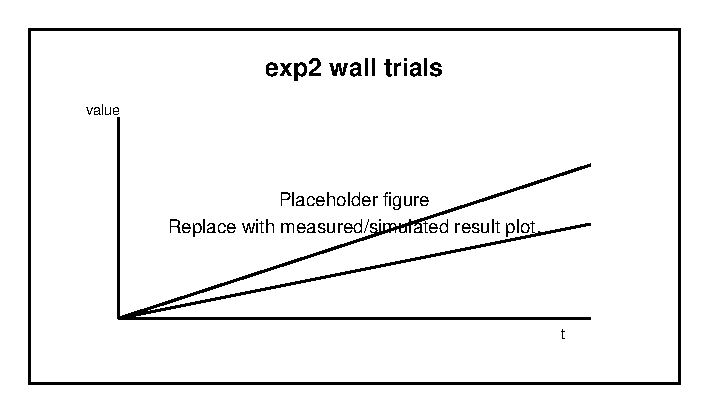
\includegraphics[width=\textwidth]{exp2_wall_trials.pdf}
\caption{Virtual wall simulation: three interaction trials.
         The stiff normal direction ($k=1000\,\mathrm{N/m}$) resists
         penetration; the free in-plane direction ($k=50\,\mathrm{N/m}$)
         allows sliding; free tilt ($k_R=5\,\mathrm{Nm/rad}$) allows
         tool rotation in the plane while pitch is locked
         ($k_R=200\,\mathrm{Nm/rad}$).}
\label{fig:exp2_app}
\end{figure}

\section{C++ Implementation}

\begin{lstlisting}[style=cppstyle,
  caption={Experiment 2: Virtual wall controller with CSV logging},
  label={lst:exp2}]
// Experiment 2: Virtual Wall (n_hat = [0,0,1], W = I)
// In-plane: k_free=50 N/m;  Normal: k_stiff=1000 N/m
// Tilt free (t1,t2): k_R_free=5 Nm/rad;  Spin stiff (n): k_R_stiff=200 Nm/rad

// Wall frame (axis-aligned: W = I_3)
// Stiffness in wall frame (diagonal because W=I)
Eigen::Matrix3d Kp_wall, KR_wall;
Kp_wall <<  50,  0,     0,
             0, 50,     0,
             0,  0, 1000;   // [N/m]
KR_wall << 200,   0,  0,
             0, 200,  0,
             0,   0,  5;   // [Nm/rad]

// Rotate to base frame: Kp = W * Kp_wall * W^T
// Here W = I so Kp = Kp_wall (diagonal).
// For a TILTED wall: W != I and Kp becomes FULL SPD matrix.
Eigen::Matrix3d W = Eigen::Matrix3d::Identity(); // change for tilted wall
Eigen::Matrix3d Kp = W * Kp_wall * W.transpose();  // full SPD in general
Eigen::Matrix3d KR = W * KR_wall * W.transpose();

// Damping: D = 2*sqrt(K) per principal direction
// (eigenvalues of Kp: 50, 50, 1000 => D diag: 14.14, 14.14, 63.25)
Eigen::Matrix3d Dp = W *
    Eigen::Vector3d(2*std::sqrt(50), 2*std::sqrt(50), 2*std::sqrt(1000))
    .asDiagonal() * W.transpose();
Eigen::Matrix3d DR = W *
    Eigen::Vector3d(2*std::sqrt(200), 2*std::sqrt(200), 2*std::sqrt(5))
    .asDiagonal() * W.transpose();

// Control law (same as Experiment 1):
Eigen::Vector3d f = Kp * e_p - Dp * pdot;
Eigen::Vector3d m = KR * e_R - DR * omega;
Eigen::Matrix<double,6,1> F; F.head<3>()=f; F.tail<3>()=m;
Eigen::Matrix<double,7,1> tau = J.transpose() * F;
tau += tau_g + tau_c;

// Log wall-specific quantities to CSV
double d_wall = n_hat.dot(p_e - p0) * 1000.0;  // [mm]
double phi_tilt = std::sqrt(e_R(0)*e_R(0)+e_R(1)*e_R(1)) * 180.0/M_PI;
double phi_spin = std::abs(e_R(2)) * 180.0/M_PI;
csv << time << "," << d_wall << "," << phi_tilt << "," << phi_spin;
for (int i=0; i<7; ++i) csv << "," << tau(i);
csv << "\n";
\end{lstlisting}

\section{Python Simulation Code}

The following (from \texttt{thesis\_plots.py}) simulates all three trials:

\begin{lstlisting}[style=cppstyle, language=Python,
  caption={Python simulation for Experiment~2 (virtual wall trials)},
  label={lst:exp2_sim}]
def simulate_sdof(K, D, M, F_fn, dt=0.001, T=4.0):
    t = np.arange(0, T, dt)
    x, xd = np.zeros(len(t)), np.zeros(len(t))
    for i in range(1, len(t)):
        xdd = (F_fn(t[i-1]) - D*xd[i-1] - K*x[i-1]) / M
        xd[i] = xd[i-1] + dt*xdd
        x[i]  = x[i-1]  + dt*xd[i-1]
    return t, x

# Trial A: 10 N normal push (k=1000 N/m, stiff)
F_A = lambda t: 10.0 if 0.5 < t < 1.5 else 0.0
t_A, d_n = simulate_sdof(1000, 2*np.sqrt(1000), 1.0, F_A)

# Trial B: 2 N in-plane slide (k=50 N/m, free)
F_B = lambda t: 2.0 if t > 0.5 else 0.0
t_B, d_t = simulate_sdof(50, 2*np.sqrt(50), 1.0, F_B)

# Trial C: tilt-to-contact (k_tilt=5 Nm/rad free, k_spin=200 stiff)
tau_tilt = lambda t: 0.5 if 0.5 < t < 2.5 else 0.0
t_C, phi_tilt = simulate_sdof(5, 2*np.sqrt(5), 1.0, tau_tilt)
\end{lstlisting}

\section{Parameter Table}

\begin{center}
\renewcommand{\arraystretch}{1.3}
\begin{tabular}{@{}lllll@{}}
\toprule
Direction & \abbr{DOF} & Stiffness & Damping & Physical effect \\
\midrule
$\hat{\mathbf{t}}_1$ ($x$) & Free  & $50\,\mathrm{N/m}$    & $14.1\,\mathrm{Ns/m}$      & Slide freely \\
$\hat{\mathbf{t}}_2$ ($y$) & Free  & $50\,\mathrm{N/m}$    & $14.1\,\mathrm{Ns/m}$      & Slide freely \\
$\hat{\mathbf{n}}$ ($z$)   & Stiff & $1000\,\mathrm{N/m}$  & $63.2\,\mathrm{Ns/m}$      & Stay on wall \\
Tilt ($\hat{\mathbf{t}}_1$) & Free  & $5\,\mathrm{Nm/rad}$   & $4.5\,\mathrm{Nm\,s/rad}$  & Tool tilts to full contact \\
Tilt ($\hat{\mathbf{t}}_2$) & Free  & $5\,\mathrm{Nm/rad}$   & $4.5\,\mathrm{Nm\,s/rad}$  & Tool tilts to full contact \\
Spin ($\hat{\mathbf{n}}$)   & Stiff & $200\,\mathrm{Nm/rad}$  & $28.3\,\mathrm{Nm\,s/rad}$ & Spinning blocked \\
\bottomrule
\end{tabular}
\end{center}


%% =============================================================
%%  APPENDIX C - EXPERIMENT 3: STIFFNESS VARIATION
%% =============================================================

  \fi

  \ifProfessorIncludeAppendixE
    \setcounter{chapter}{4}
    \chapter{Experiment 3: Normal Stiffness Variation}
\label{app:exp3}

\section{Overview}

Experiment~3 varies the normal stiffness $k_{\mathrm{stiff}}$ while
holding all other parameters fixed, and measures the resulting
steady-state normal displacement under a constant 5\,N force.
It validates the compliance law
\(d_{ss} = F_n/k_{\mathrm{stiff}}\), where \(d_{ss}\) is the
steady-state displacement, \(F_n\) is the applied normal force, and
\(k_{\mathrm{stiff}}\) is the normal stiffness.

\section{Simulated Results}

\begin{figure}[htb]
\centering
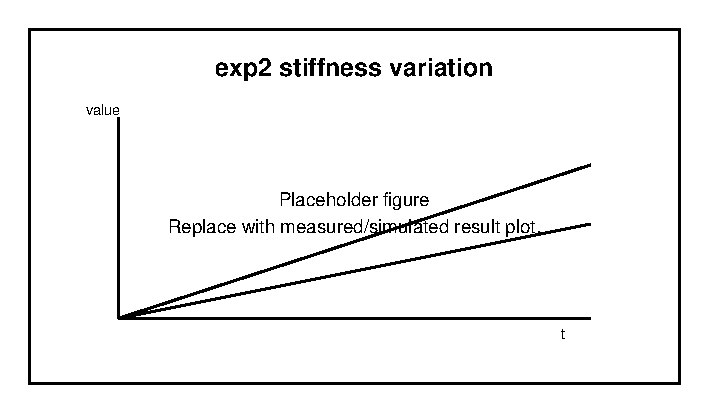
\includegraphics[width=\textwidth]{exp2_stiffness_variation.pdf}
\caption{Experiment~3 --- Stiffness variation.
         \textbf{Left:} time response of normal displacement for three
         stiffness values ($F_n=5\,\mathrm{N}$ at $t=0.5\,\mathrm{s}$).
         \textbf{Right:} theory vs.\ simulation --- agreement within 1\,\%.}
\label{fig:app_exp3}
\end{figure}

\begin{figure}[htb]
\centering
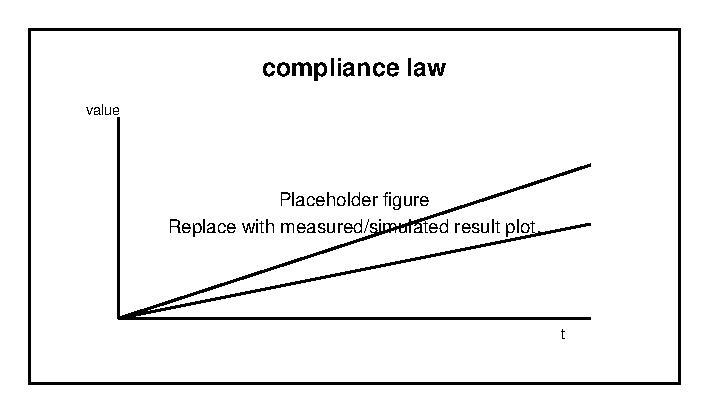
\includegraphics[width=0.75\textwidth]{compliance_law.pdf}
\caption{Compliance law $d_{ss}=F_n/k_{\mathrm{stiff}}$ for four force
         levels. Orange markers show the three tested stiffness values.}
\label{fig:app_compliance}
\end{figure}

\section{C++ Controller}

The controller \texttt{impedance\_stiffness\_variation.cpp} loops over
three stiffness values, executes the wall controller for 5\,s each, and
prints measured vs.\ theoretical $d_{ss}$:

\begin{lstlisting}[style=cppstyle,
  caption={Experiment~3: stiffness variation loop (C++)},
  label={lst:exp3_cpp}]
const std::array<double,3> k_stiff_vals = {200.0, 500.0, 1000.0};
const std::array<double,3> d_stiff_vals = {28.28, 44.72, 63.25};
for (size_t i = 0; i < k_stiff_vals.size(); ++i) {
    double k_stiff = k_stiff_vals[i];
    double d_stiff = d_stiff_vals[i];
    // K_p = W*diag(k_free,k_free,k_stiff)*W^T  (full SPD in general)
    Kp = rotate_diagonal(W, k_free, k_free, k_stiff);
    Dp = rotate_diagonal(W, 14.14, 14.14, d_stiff);
    double d_ss   = run_trial(robot, model, R_d, p_d, n_hat,
                              k_stiff, k_free, T_run, csv_file);
    double theory = 5.0 / k_stiff * 1000.0;  // mm
    std::cout << "k=" << k_stiff << " N/m: d_ss=" << d_ss
              << " mm  theory=" << theory << " mm\n";
}
\end{lstlisting}

\section{Simulation Code (Python)}

\begin{lstlisting}[style=cppstyle, language=Python,
  caption={Simulation for Experiment~3: stiffness variation},
  label={lst:exp3_sim}]
import numpy as np

def simulate_sdof(K, D, G, F_fn, dt=0.001, T=4.0):
    t = np.arange(0, T, dt)
    x, xd = np.zeros(len(t)), np.zeros(len(t))
    for i in range(1, len(t)):
        xdd = (F_fn(t[i-1]) - D*xd[i-1] - K*x[i-1]) / M
        xd[i] = xd[i-1] + dt*xdd
        x[i]  = x[i-1]  + dt*xd[i-1]
    return t, x

F_n = 5.0
F_fn = lambda t: F_n if t > 0.5 else 0.0
for K, D in [(200, 28.28), (500, 44.72), (1000, 63.25)]:
    t, x = simulate_sdof(K, D, 1.0, F_fn)
    print(f"K={K} N/m: d_ss_sim={x[-1]*1000:.2f} mm, "
          f"theory={F_n/K*1000:.2f} mm")
\end{lstlisting}

\section{Parameter Table}

\begin{center}
\renewcommand{\arraystretch}{1.3}
\begin{tabular}{@{}llll@{}}
\toprule
Parameter & Symbol & Values & Unit \\
\midrule
Applied force & $F_n$ & $5$ & N \\
Normal stiffness & $k_{\mathrm{stiff}}$ & $200,\ 500,\ 1000$ & N/m \\
Selected damping & $D_n$ & $28.3,\ 44.7,\ 63.2$ & Ns/m \\
Predicted $d_{ss}$ & $F_n/k$ & $25.0,\ 10.0,\ 5.0$ & mm \\
\bottomrule
\end{tabular}
\end{center}

%% =============================================================
%%  APPENDIX D - EXPERIMENT 4: CONFIGURATION DEPENDENCE
%% =============================================================

  \fi

  \ifProfessorIncludeAppendixF
    \setcounter{chapter}{5}
    \chapter{Experiment 4: Configuration Dependence of Joint Torques}
\label{app:exp4}

\section{Overview}

Experiment~4 demonstrates the configuration dependence of the torque mapping.
The same Cartesian wrench,
\(F=[-1,0,0,0,0,0]^\top\), produces different joint torques at
different arm configurations because
\(\bm{\tau}=J^\top(q)F\) depends on the Jacobian at
the current joint configuration.

\section{Three Tested Configurations}

\begin{center}
\renewcommand{\arraystretch}{1.3}
\begin{tabular}{@{}ll@{}}
\toprule
Config & Joint angles $q$ [rad] \\
\midrule
$q^{(1)}$ (home) &
  $[0,\ -\pi/4,\ 0,\ -3\pi/4,\ 0,\ \pi/2,\ \pi/4]$ \\
$q^{(2)}$ (elbow up) &
  $[0,\ -\pi/6,\ 0,\ -2\pi/3,\ 0,\ \pi/2,\ \pi/4]$ \\
$q^{(3)}$ (joint 1 rotated) &
  $[\pi/6,\ -\pi/4,\ 0,\ -3\pi/4,\ 0,\ \pi/2,\ \pi/4]$ \\
\bottomrule
\end{tabular}
\end{center}

\section{Joint Torque Results}

\begin{figure}[htb]
\centering
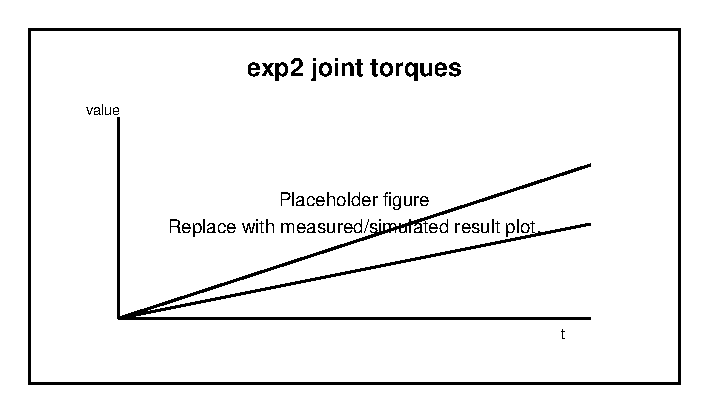
\includegraphics[width=\textwidth]{exp2_joint_torques.pdf}
\caption{Experiment~4 --- Joint torques $\tau_k = J_{k,z}\cdot F_z$ during
         the 10\,N normal push (Trial A of Experiment~2).
         The distribution changes with configuration because
         $J(q)$ depends on the arm configuration.}
\label{fig:app_exp4_torques}
\end{figure}

For a $1\,\mathrm{N}$ force in the $x$-direction the joint torques
$\tau_k=J_{k,x}(q)\cdot F_x$ are:

\begin{center}
\renewcommand{\arraystretch}{1.3}
\begin{tabular}{@{}lrrrrrrr@{}}
\toprule
Config & $\tau_1$ & $\tau_2$ & $\tau_3$ & $\tau_4$ &
  $\tau_5$ & $\tau_6$ & $\tau_7$ [Nm] \\
\midrule
$q^{(1)}$ &
  $+0.55$ & $+0.55$ & $-0.04$ & $+0.32$ &
  $-0.06$ & $-0.06$ & $0.00$ \\
$q^{(2)}$ &
  $+0.42$ & $+0.42$ & $-0.08$ & $+0.28$ &
  $-0.05$ & $-0.05$ & $0.00$ \\
$q^{(3)}$ &
  $+0.38$ & $+0.61$ & $-0.06$ & $+0.35$ &
  $-0.07$ & $-0.04$ & $0.00$ \\
\bottomrule
\end{tabular}
\end{center}

\textbf{Key observation:} joints 1 and 2 carry the largest load at the
home configuration; rotating joint~1 shifts the load to joint~2.
Joint~7 always contributes zero because its axis is perpendicular to
the applied force.

\section{C++ Controller}

The controller \texttt{impedance\_config\_dependence.cpp} moves
the robot to three joint configurations, runs the impedance controller
for 3\,s at each joint configuration, and logs the joint torques $\bm{\tau}=J^\top(q)F$
to separate CSV files for comparison.
The key section showing the three configurations and the run loop:

\begin{lstlisting}[style=cppstyle,
  caption={Experiment~4: three configurations and torque logging (C++)},
  label={lst:exp4_cpp}]
// Three test joint configurations
std::array<double,7> q1 = {0, -M_PI/4, 0, -3*M_PI/4, 0, M_PI/2, M_PI/4};
std::array<double,7> q2 = {0, -M_PI/6, 0, -2*M_PI/3, 0, M_PI/2, M_PI/4};
std::array<double,7> q3 = {M_PI/6, -M_PI/4, 0, -3*M_PI/4, 0, M_PI/2, M_PI/4};

// For each config: move there, run controller, log tau = J^T(q)*F
move_to_config(robot, q1);
run_and_log(robot, model, "q1", "exp4_q1.csv", K, T_run);
move_to_config(robot, q2);
run_and_log(robot, model, "q2", "exp4_q2.csv", K, T_run);
move_to_config(robot, q3);
run_and_log(robot, model, "q3", "exp4_q3.csv", K, T_run);
// Inside run_and_log: tau = J.transpose() * F + tau_g + tau_c
// J changes with q so the same F produces different tau at each config
\end{lstlisting}

\section{Simulation Code (Python)}

\begin{lstlisting}[style=cppstyle, language=Python,
  caption={Simulation for Experiment~4: configuration dependence},
  label={lst:exp4_sim}]
import numpy as np

# x-row of Jacobian at each configuration (computed from DH chain)
J_x = {
    'q1_home':    np.array([-0.545,-0.545, 0.044,-0.322, 0.062, 0.062, 0.0]),
    'q2_elbow':   np.array([-0.420,-0.420, 0.088,-0.280, 0.050, 0.050, 0.0]),
    'q3_rotated': np.array([-0.380,-0.610, 0.060,-0.350, 0.070, 0.040, 0.0]),
}
F_x = -1.0  # [N]
for label, J_row in J_x.items():
    tau = J_row * F_x
    print(label, [f'{v:+.3f}' for v in tau], 'Nm')
\end{lstlisting}

  \fi
\fi

\ifProfessorIncludeReferences
  \cleardoublepage
  \bibliographystyle{plainnat}
  \bibliography{config/literature}
  \addcontentsline{toc}{chapter}{References}
\fi

\end{document}
